\chapter{Finding faster configurations using flash}
\label{chapter:flash}

This chapter presents an approach to estimating end-to-end performance
of distributed storage systems.
We explain why low-level performance metrics are a desirable proxy
for estimating end-to-end performance.
We then present our automatic model building tool for generating
robust and accurate performance models.

% \section{Introduction}
\label{ch4:sec:introduction}

Many storage systems are moving away from dedicated appliance-based storage model to software-defined 
storage (SDS), which separates software that provisions and manages storage from the hardware that provides raw physical storage~\cite{sds_att, Thereska2013, Jalaparti2012}.
This trend is partly driven by the tremendous growth of data and the emergence of cloud applications that operate in a multi-tenant environment with diverse workload characteristics.
As a result, the rigid appliance-based model, with tightly-coupled hardware and software features, is no longer cost-effective, lacks flexibility, and does not scale well.
SDS systems are increasingly abandoning centralized storage services in favor of distributed systems like Ceph~\cite{ceph}, HDFS~\cite{hadoop}, Swift~\cite{openstack}. 
Distributed storage systems are attractive because they scale well, allowing storage services to grow or shrink, based on storage demands. 
They are also better suited to handle diverse multi-tenant workloads. 

Providing reliable quality of service (QoS) to storage applications is critical in an SDS environment shared by multiple applications 
with diverse usage patterns. However, in a distributed storage environment, it is challenging to provide storage QoS in a consistent 
and reliable manner. Practical deployments of modern distributed storage systems like Ceph are composed of a large number of 
individual storage components that can interact in a complex manner. 
Diverse and time-varying storage workloads and performance interference in a multi-tenant environment further 
complicate the reliable assurance of storage QoS. Reliable and accurate monitoring of 
high-level storage performance metrics (e.g. throughput and IOPS) is critical 
for providing storage QoS guarantees.    
However, monitoring end-to-end storage performance is difficult in a distributed storage service. 
Instrumenting user applications to measure storage performance is not always practical. 
Performing benchmark tests in production systems also has practical limitations since they 
interfere with storage application workload.
Furthermore, running exhaustive benchmark experiments to cover diverse application workloads, 
deployment topologies, and large configuration parameter space is time-consuming and impractical in many cases. 
Building accurate analytical performance models, on the other hand, is also difficult for the reasons mentioned above.
 
This chapter proposes the idea of using low-level system metrics (e.g., CPU usage, RAM usage and network I/O)
as a proxy for measuring high-level performance (e.g., end-to-end IOPS and throughput) of 
distributed storage applications.
We design, implement and evaluate a practical tool, called \emph{Inside-Out}, that applies 
machine learning techniques to the low-level metrics collected from individual components 
of a distributed storage system to accurately estimate high-level storage performance metrics---like throughput and IOPS---of the entire 
distributed storage system.
We believe that a tool like Inside-Out can serve as an important component of the overall SDS architecture.

Inside-Out takes a black-box modeling approach, which does not require knowledge about distributed storage system protocol, workload characteristics, and deployment topology. 
Inside-Out relies upon machine learning techniques to automatically derive an accurate end-to-end performance model.
We explore several well-known machine learning algorithms including linear regression, 
decision tree learning, and ensemble methods \cite{Wang2004, Noorshams2013}, and conclude that  
there does not exist an one-size-fits-all algorithm that can work in all prediction cases.
Hyperparameter tuning \cite{Chapelle2002, Noorshams2013}, model selection \cite{Kohavi1995} and 
feature selection \cite{guyon2003introduction, Saeys12007} all turn out to be too complicated for optimizing prediction accuracy.
In contrast, Inside-Out uses a two-level learning method that automatically selects important features, boosts prediction accuracy, and achieves consistent prediction. 
This two-level learning method pipelines two supervised learning algorithms to eliminate irrelevant features while avoiding overfitting problems.\footnote{\label{ft:overfitting}
Overfitting describes the situation when a model captures the relationship of noisy data but not the underlying relationship \cite{domingos2012few}.
Overfitting becomes more prominent in the presence of high dimensional data}

Inside-Out offers several key benefits. 
%[MRA] Unlike traditional analytic performance modeling approach, Inside-Out is generic in nature, and therefore, it can be applied to different storage services.  
Unlike traditional analytic performance modeling approach, Inside-Out is more generic, 
and therefore can be more easily applied to different storage services.  
Different from previous work, Inside-Out 
does not require information about system configuration and application workload~\cite{Ruemmler1994, Shriver1998, Wang2004, Kelly2004, Yin2006, Noorshams2013, Ardagna2014}. 
Due to the self-learning property, \emph{Inside-Out} improves performance prediction accuracy with more data.
It can also adapt to changes in the system
by continuously learning the system behavior. 

We evaluate Inside-Out using Ceph~\cite{ceph} %as an example distributed storage system 
running on an OpenStack-based SDS platform.
The low-level performance metrics are collected from participant virtual machines 
running various components of a Ceph storage service.\footnote{\label{ft:vm}
Our approach is not limited to VM-based environments.
It can be applied to container-based and bare-metal storage servers as well.
}
Our in-depth evaluation shows that Inside-Out generates end-to-end performance models with 91.1\% prediction accuracy on average.
More importantly, as discussed above, Inside-Out is generic in nature as it captures the behavior of the storage system 
by analyzing low-level system metrics (that are protocol and application agnostic). Furthermore, we demonstrate that Inside-Out 
%[MRA] can provide reliable performance monitoring even in the presence of evolving workload characteristics, changing storage 
can provide reliable hints for performance monitoring tasks even in the presence of evolving workload characteristics, changing storage 
configuration and interfering tenants. We also show that Inside-Out is reliable in estimating end-to-end performance 
even when the storage system expands or shrinks.
We show that Inside-Out provides reliable performance 
prediction when the storage system is up to four times larger than the one used for building machine learning models during 
the training phase. 
Lastly, Inside-Out is able to learn new storage behavior over time.
% \section{Mapping from Low to High}
\label{sec:challenges}

%[commented by MRA] We discuss how to use low-level performance metrics collected from distributed components to build an accurate end-to-end performance model for a distributed storage system in the SDS environment.
This section discusses the guiding principles and challenges in using low-level performance metrics
to build accurate end-to-end performance models for a distributed storage system.
%collected from individual components of a 
%distributed storage system for building an accurate end-to-end performance model.

%\subsection{Searching for Representative Features}
\subsection{Important Considerations}

This section describes how we use low-level performance metrics
to predict high-level system performance.
We discuss how we pick the metrics and how to transform metrics
to meaningful features.

\label{sec:feaatures_for_distributed_system}

%[commented by MRA] We have to keep in mind that we are developing a tool that can apply to diverse storage services to be deployed in SDS.
%Manually building models for each storage service requires energy and cost that are several times more than an automatic and general approach.
%Note that we are developing a tool that can be applied to a diverse set of storage systems and services.
%Manually building a model for each storage service requires more effort and cost compared to an automated 
%and general, i.e., application-agnostic, approach.

%\subsubsection{Requiring general performance metrics}
\subsubsection*{General low-level metrics}
%
%Low-level performance metrics are general and application independent.
Since our goal is to provide a tool for estimating the end-to-end performance of a diverse set of 
storage systems, the inputs to our model need to be generic in nature, \ie they need to 
be independent of storage systems or the distributed protocols used by such applications. An SDS provider 
should be able to obtain the input metrics without instrumenting storage application or requiring domain 
knowledge about the storage application. Low-level system metrics (e.g. CPU utilization, memory usage, network IO, etc.) 
satisfy these requirements. DeepDive uses low-level metrics to identify performance anomaly for a running VM~\cite{Novakovic2013}. 
To the best of our knowledge, this work presents the first study that maps low-level system metrics to 
high-level end-to-end performance of a distributed storage service.

%Low-level performance metrics are application independent.
%An SDS provider can obtain this information without instrumenting applications.
%For example, DeepDive~\mra{citation?} use low-level metrics to identify performance anomaly for a running VM \cite{Novakovic2013}.
%To the best of our knowledge, this paper presents the first study that maps low-level performance metrics to high-level end-to-end performance of a distributed storage service.

\begin{figure}
\centering
\includegraphics[width=0.9\textwidth, keepaspectratio]{figures/features.pdf}
\caption{Four statistical features used in Inside-Out to capture load and internal status of a distributed storage system.  The numbers and metrics represent low-level performance data collected from storage nodes.}
\label{fig:feature_types}
\end{figure}


%\subsubsection{Handling the distributed system scenario}
\subsubsection*{Capture important features of a distributed storage system}
%
%One important characteristic of a distributed storage system is that it can expand or shrink on demand 
A distributed storage system can dynamically expand or shrink
according to demand.
The performance model has to capture the current 
scale of the deployment, the bottlenecks, and the average and variance in performance
of individual components of the distributed system. For each low-level system metric collected from 
various components of the distributed system, we use four statistical variables to characterize the behavior of a distributed system (see \myfigure{\ref{fig:feature_types}}). 
The statistical variable \textit{mean} and \textit{std} describe whether the impact of the workload is evenly distributed among 
storage components. The \textit{sum} variable represents the scale of the deployment, while the variable \textit{5\%} (top 5 percentile) captures the hot spot situations. 
The feature transformation from raw system metrics to these four statistical values also allows Inside-Out to apply 
the uniform input format for developing performance models for distributed systems at different scales.

\subsection{Feature Selection}
\label{sec:non-deterministic}

In this work, we collect low-level performance metrics
from two components of Ceph
namely monitor (MON) and Object Storage Daemons (OSD).
We use \emph{dstat}, a monitoring tool to collect resource statistics,
to collect 32 low-level performance metrics in total.
These measurements are then transformed using the process described in \myfigure{\ref{fig:feature_types}} (refer to Section~\ref{sec:data_preprocessing} for more details).


Selecting the ``right'' features from high dimensional data
is a challenging task because
as computation complexity increases, prediction accuracy may decreases
~\cite{guyon2003introduction, Saeys12007}.
Furthermore, for our case, the right feature set is not always the identical.
Table \ref{tab:challenge_feature_selection} shows the \emph{model accuracy} of different learning methods when modeling 
read throughput. 
%\chin{
%verified with $10$-fold cross validation.
%}
We see that all learning methods achieve high model accuracy
even though they choose different features. 
The model accuracy was obtained using $k$-fold cross validation (\textit{k}=10),
a common technique for assessing model accuracy. 
The training data is partitioned into $k$ disjoint sets. 
A single data partition is used for validation purpose and the remaining $k-1$ partitions are used for training data.
Although all models yield good model accuracy, they perform poorly and inconsistently when the storage environment changes. 
In \myfigure{\ref{fig:challenge_generalization}},
we show the prediction accuracy under
%we show prediction accuracy when we make
three types of changes in the storage environment---increase in the size of the distributed 
storage system, read workload and individual storage IO request size.
These algorithms (discussed later in Section~\ref{sec:algorithm_selection}) do not yield consistent prediction accuracy any more. 
For example, Lasso can still predict well when workload has changed but Decision Tree cannot.
On the contrary, Decision Tree performs better than Lasso when the size of the storage system increases.
We suspect this is caused by the large feature space, which leads to the overfitting problem \cite{domingos2012few, hastie2005}.
Next, we manually remove most features and select only a few with a trial-and-error strategy.
As shown in \myfigure{\ref{fig:challenge_generalization}}, we see significant improvement in some cases, but not all. 
Since an SDS environment can change over time, it is important for our model to provide consistent prediction accuracy under system changes
such as software reconfiguration and cluster expansion.


\begin{table*}[t!]
\caption{Important features selected by different algorithms are not deterministic}
\centering
\label{tab:challenge_feature_selection}
%\begin{tabular}{|lll|lll|lll|lll|lll|}
%\resizebox{!}{.8\linewidth}{
\resizebox*{\textwidth}{!}{
\begin{tabular}{|lll|lll|lll|lll|lll|}
%\begin{tabularx}{1.0\linewidth}{|lXl|lXl|lXl|lXl|lXl|}

\hline
\multicolumn{3}{|c|}{\textbf{Lasso}}   & \multicolumn{3}{c|}{\textbf{Ridge}}   & \multicolumn{3}{c|}{\textbf{Elastic Net}} & \multicolumn{3}{c|}{\textbf{Decision Tree}} & \multicolumn{3}{c|}{\textbf{Random Forest}} \\
\hline
osd  & network.send  & sum  & \textbf{osd}  & \textbf{network.recv}  & \textbf{mean} & osd   & network.send   & sum    & osd    & disk.read       & sum    & osd    & disk.read       & sum    \\
osd  & disk.writ     & sum  & \textbf{osd}  & \textbf{disk.read}     & \textbf{5\%}  & osd   & disk.writ      & sum    & osd    & network.send    & sum    & osd    & network.send    & sum    \\
\textbf{osd}  & \textbf{cpu.sys}       & \textbf{sum}  & \textbf{osd}  & \textbf{load.15m}      & \textbf{std}  & osd   & disk.read      & sum    & osd    & network.recv    & sum    & osd    & disk.writ       & sum    \\
osd  & io.read       & sum  & osd  & network.send  & sum  & osd   & cpu.sys        & sum    & osd    & disk.writ       & sum    & \textbf{osd}    & \textbf{network.recv}    & \textbf{sum}    \\
osd  & vm.minpf      & mean & osd  & tcp.tim       & std  & osd   & tcp.lis        & sum    & \textbf{mon}    & \textbf{memory.buff}     & \textbf{mean}   & osd    & memory.cach     & sum    \\
\textbf{mon}  & \textbf{memory.used}   & \textbf{5\%}  & osd  & network.recv  & std  & osd   & io.read        & std    & osd    & cpu.sys         & sum    & osd    & memory.buff     & mean   \\
\textbf{mon}  & \textbf{memory.cach}   & \textbf{5\%}  & osd  & load.5m       & std  & osd   & io.read        & sum    & osd    & vm.alloc        & sum    & osd    & memory.buff     & 5\%    \\
osd  & tcp.lis       & sum  & osd  & cpu.idl       & sum  & osd   & vm.minpf       & mean   & osd    & vm.minpf        & 5\%    & mon    & io.writ         & sum    \\
osd  & io.read       & std  & osd  & cpu.wai       & sum  & osd   & io.writ        & mean   & \textbf{mon}    & \textbf{cpu.idl}         & \textbf{std}    & osd    & memory.buff     & sum    \\
osd  & io.writ       & mean & osd  & cpu.sys       & sum  & \textbf{mon}   & \textbf{memory.used}    & \textbf{sum}    & mon    & memory.cach     & sum    & mon    & vm.free         & sum    \\
\hline
\multicolumn{3}{|c|}{96.20\%} & \multicolumn{3}{c|}{96.60\%} & \multicolumn{3}{c|}{96.18\%}     & \multicolumn{3}{c|}{96.78\%}       & \multicolumn{3}{c|}{96.94\%} \\
\hline
\end{tabular}
%\end{tabularx}
}
\end{table*}



\begin{figure*}
    \centering
    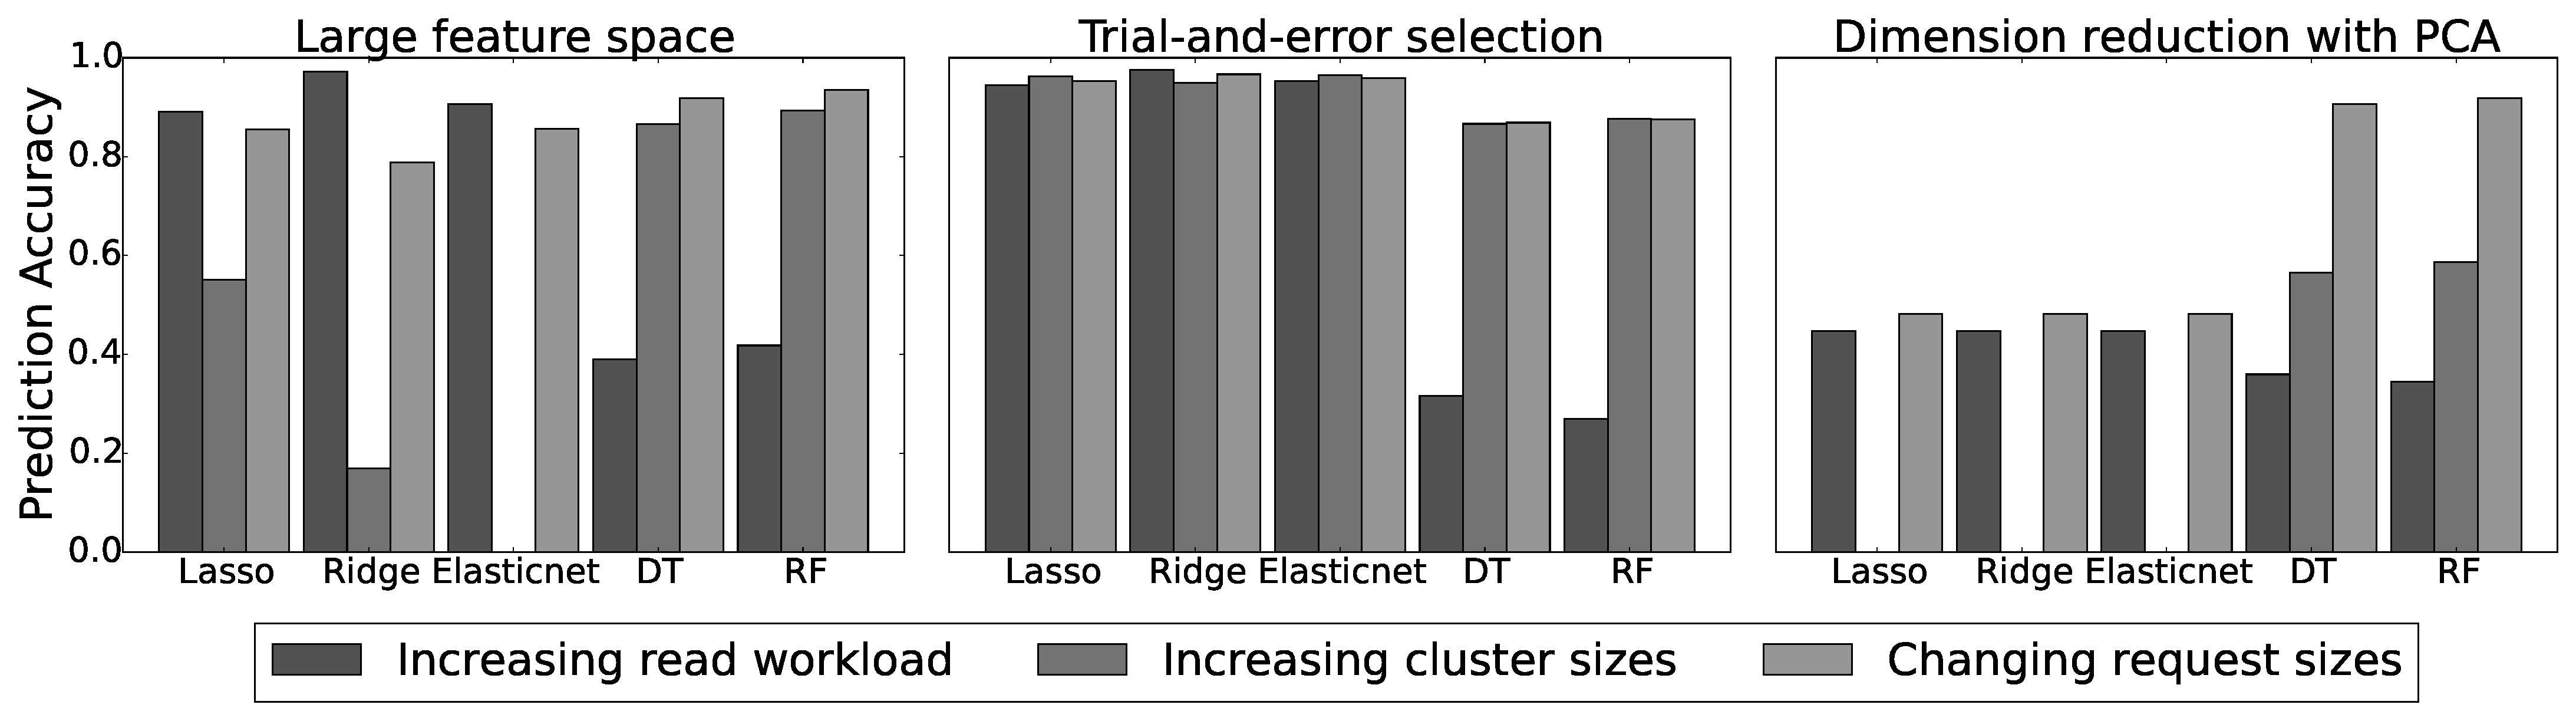
\includegraphics[width=1\textwidth]{figures/challenge_generalization_combined_horizental.eps}
    \caption{Prediction accuracy is inconsistent due to the large feature space.
    Learning methods fail to select the right features in some cases.
    Dimension reduction (PCA with 10 components) does not help in this case.
    In the trial-and-error case, we select a subset of metrics, e.g. \emph{mean(disk.read)}, \emph{sum(network.recv)} and \emph{std(cpu.usr)}.}
    \label{fig:challenge_generalization}
\end{figure*}

Although Hyperparameter tuning, model selection, and 
feature selection have been proposed as potential solutions, it is challenging 
to use them in practice, not to mention the complexity of automating this task. 
PCA (Principle Component Analysis) is another potential solution \cite{Shlens2003}.
PCA transforms original data into a lower dimension while keeping high fidelity.
However, PCA has several limitations. 
First, PCA is not scale invariant.
Not all performance metrics are comparable and therefore, there is no standard way to scale these metrics.
Second, PCA assumes Gaussian distribution in data points; however, many storage workloads have Pareto distribution \cite{Kim2010}.
Third, determining a good number of components is also a challenging task.
In our case, PCA does not address the problems.
In fact, \myfigure{\ref{fig:challenge_generalization}} shows that it can further degrade prediction accuracy.

\subsection{A Two-Level Approach}

Instead of performing feature selection or dimension reduction, we propose a generic two-step approach that can improve the consistency of prediction accuracy. 
In the first step, we use some heuristic methods to filter out irrelevant features.
Then, in the second step, we apply machine learning algorithms to build performance models with the reduced feature set.
The intuition behind this idea is that it is difficult to determine the most important performance features but it is relatively easy to eliminate unimportant features.
For example, the features which are not in the top 100 list after step one can be labeled as unimportant features.
% \section{The Inside-Out Design}
\label{sec:methodology}
%\rp{Chin: In the previous section, you say ``As we will explain in Section V-A, we use 32 low-level performance 
%metrics collected with dstat''. This section does not say anything about 32 metrics. Please mention them here. 
%I think we need to write this section in a much better way. You should clearly explain the steps: something like: We collect 32 
%low level system metrics from each VM (either give the list or mention just the few) every x seconds. Then say we take mean, std, sum and 5\% of each 
%of these 32 metrics for every moving window of xxx seconds. Then explain why we use moving window. then say that for training and validation purposes, 
%we measure the end-to-end performance metrics (IOPS, throughput, and latency) using cosbench every x seconds. Then we take average, xxx, xxx etc. 
%of these metrics ...I think you get the point now, right? We have to clearly explain what we exactly did. }
In this section, we present the design of Inside-Out.
We also discuss the trade-offs among a set of representative machine learning algorithms
and propose a two-step learning technique for mitigating overfitting problems.



\subsection{Collecting and Pre-Processing Low-Level Metrics}
\label{sec:data_preprocessing}

Inside-Out collects general, low-level system metrics from individual machines running the distributed storage service.
However, the raw collected data suffers from various problems due to inefficiency of data collectors, system clock skews,
incomparable data formats, workload outliers, bursty system anomalies, \etc
The noisy data can lead to unstable and 
inaccurate performance models. 
Inside-Out performs a series of data pre-processing functions to address these issues.

%\rp{The goal of this step is to remove unwanted characteristics of the collected data, such as
%workload outliers, system clock deviation, incomparable data format, etc.
%}


%Data preprocessing is a preparation step before training a model.


\subsubsection{Monitoring storage components}
We collect low-level system metrics of the underlying operating system to capture resource utilization 
(\eg cpu, memory, disk and network usage).  
The low-level performance metrics are sampled with one-second granularity.
Such data can be collected from \textit{libvirt}, Ganglia, instrumented hypervisors \cite{Koh2007} and \textit{Ceilometer} in OpenStack.
We use  \emph{dstat} monitoring tool (with option: -tcly -mg --vm -dr -n --tcp --float) to collect these data.


%This step helps us eliminate unwanted characteristics of the collected data, such as
%high variation due to workloads, uncertainty originated by physical hardware, 
%system clock deviation, incomparable data format, etc.
%For the collected performance data, fluctuating metrics, time synchronization and feature transformation for a distributed system are the major challenges.

%\subsubsection{Smoothing monitored data}
\subsubsection{Data smoothing}
%
Building a performance model with data collected at one-second granularity is challenging because 
system data can exhibit high variance at small time scales, \eg due to dynamic/bursty workloads and interference among co-located tenants.
Furthermore, the storage IO operation needs to pass through a series of software layers 
between the storage client and the back-end raw physical storage device. 
The long storage IO path can introduce high variability in resource utilization at smaller time scales. 
For example, HDFS and Ceph both replicate data blocks across storage nodes distributed in physically disjoint 
servers, racks or even datacenters.
To address the uncertainties due to complex IO path spanning several software layers, 
we compute the moving average of the collected performance data.
We have empirically found that one-minute window for processing the moving average is sufficient to 
eliminate outliers from the raw data.
%we use moving averages to construct a stable prediction model.
%We choose one-minute windows for moving average since we have empirically found 60-second moving averages to smooth out raw data sufficiently, without 
%compromising data quality, in order to yield stable and accurate performance models.
%A fine granularity, at lease 15 seconds, is also desirable from our experience.

%RP: Chin, I commented the following line becuause it looks too vague. If you want to clarify this, 
%we can restate in a better way. 
%and the uncertainty come from the interaction between software and hardware components.
%We use moving average to smooth the collected performance data for stable prediction model.
%\rp{Chin: Please explain ``moving average of xxx'', ``why 15 seconds is a desirable window''. These aspects need to be mentioned 
%in a clear manner, not in a handwavy way.}
%We use moving average to construct a stable prediction model.
%Based on our data collected from our internal testbed, 
%it is desirable to use a window greater than 15 seconds. 
%From our experience, a window greater than 15 seconds shows stable results.
%One reason is that a storage request can last longer than 10 seconds for accessing large objects (or files).

\subsubsection{Timestamp alignment}
Proper time synchronization among participating servers is essential to correlate data collected from those servers. 
We use NTP for time synchronization.
The average timestamp of all nodes is taken as the basis for time alignment.

\subsubsection{Feature transformation for a distributed storage system}
%
As mentioned earlier, elasticity is an important feature of SDS, since it needs to adjust its size based on storage demand. 
%The built prediction model needs to be able to predict end-to-end performance at different system scales.
Thus our model must accurately predict end-to-end performance at arbitrary deployment scales.
However, the data collected from different scales may have different dimensions. 
For instance, Ceph with 10 Object Storage Servers (OSDs) generates 10 copies of low-level performance metrics, 
while Ceph with 5 OSDs generates fewer data points. This makes it hard to train and build a unified model.
As mentioned in Section~\ref{sec:feaatures_for_distributed_system}, we use \emph{mean, sum, std, and 5\%} statistical 
variables to capture 
different types of workload distribution such as
\emph{hotspot}, \emph{load imbalance}, and \emph{aggregate performance}.

%To achieve the goal, we need to make sure the dimension of data, collecting from different system configurations are comparable.
%As suggested in Section~\ref{sec:feaatures_for_distributed_system}, our feature transformation describes a distributed system as in one of the four conditions: load-balancing, non-load-balancing, hotspot and the aggregate workload.
%As suggested in Section~\ref{sec:feaatures_for_distributed_system}, our feature transformation process 
%takes four conditions into account: load-balancing, non-load-balancing, hotspot and the aggregate workload.

In summary, Inside-Out collects 32 raw low-level system metrics with one-second granularity.
Inside-Out applies proper time alignment and moving average with one-minute windows for stabilizing performance data.
Then it calculates \emph{mean}, \emph{std}, \emph{sum} and \emph{5\%} of individual metrics collected from multiple machines.
This ensures that our performance model can accept input data for systems with varying scales of deployment, 
while preserving important characteristics of a distributed storage system.
For training and validation purposes, 
we measure end-to-end performance metrics (IOPS, throughput, and latency) every 5 seconds using COSbench \cite{cosbench}, and take average over the one-minute window.
Next, we describe how we build end-to-end performance models in order to capture the relationship between low-level system metrics and end-to-end throughput and IOPS.

%Lastly, we transform low-level performance metrics to create comparable dataset while preserving characteristics 
%of a distributed storage system, using the feature transformation specified in Figure~\ref{fig:feature_types}.

%In summary, we use a 60-seconds window to smooth performance data, and proper time alignment has applied to the monitored performance data.
%\mra{Chin, what did you use to transform the data? average? It would be good if we can briefly state how we transform the data.
%if you already described this somewhere later in the paper, we could forward reference the section.}


\subsection{Exploring Learning Methods}
\label{sec:algorithm_selection}

%We collect time series data composed of low-level system metrics collected from all machines running the distributed storage system. 
%At each sampling time (every $t$ seconds), a low-level performance snapshot of a running distributed storage system is \rp{obtained from} the dataset.
%Given a performance snapshot at time $t$ of a running distributed storage, we aim to build a model that predicts the storage's end-to-end performance, e.g. throughput and IOPS.
%The performance snapshot is the low-level performance metrics collected from distributed storage nodes.

Our goal is to build a model that accurately predicts end-to-end throughput and IOPS by analyzing only the low-level metrics of a distributed storage system.
We explore several algorithms, including statistical regression \cite{Fron2004, hastie2005}, 
decision tree learning and random forests learning \cite{hastie2005,Wang2004}.
For statistical regression, we mainly focus on linear regression techniques, 
which can be extended to support non-linear regression by expanding features that simulate, 
for example, quadratic terms \cite{Kundu2010}.
We did not find this necessary in our application and exclude the discussion.

%\subsubsection{Lasso}
%\textit{Lasso\footnote{Least Absolute Shrinkage and Selection Operator}} 
% remove the full name above
\textit{Lasso} 
is a least square linear regression technique with L1-norm regularization.
The L1 penalty function leads to a sparse solution, which has an effect of restricting 
the number of selected variables.
This property is useful for figuring out important features, especially 
when the number of variables or features is large.
%
%\subsubsection{Ridge}
\textit{Ridge} is similar to Lasso but instead uses L2-norm regularization, 
which has the effect of group selection of variables.
This property does not restrict the number of variables selected by the prediction model 
and therefore, the prediction accuracy might degrade and become inconsistent 
%when the feature space is large.
when the number of input features to the training model is large. 
%when we use a small number of features out of much larger feature space.
%\mra{Chin, I modified the previous sentence. Check if it is ok with you.}
%
%\subsubsection{Elastic Net}
\textit{Elastic Net} combines both advantages---it does group selection while enforcing sparsity.
Based on our data set, Lasso and Elastic Net have similar prediction performance, and Ridge shows larger variance.
%
The \textit{Decision Tree} (DT) learning uses a top-down approach and recursively partitions data to fit target values.
The tree-based model is easy to interpret and scales well to large datasets.
\textit{Random Forests} (RF) is an ensemble method that uses multiple decision trees~\cite{hastie2005}.
%In practice, it is accurate, efficient, and more robust compared to a single decision tree.
RF improves a single decision tree in many ways, e.g., accuracy, efficiency, and robustness.
%Due to space limit, please refer to \cite{hastie2005} for detailed description.

To summarize, linear regression models assume a linear relationship and might oversimplify the storage behavior. 
Nonetheless, it has the potential to exhibit better generalization for extrapolating performance prediction 
for the unknown behavior case (the pattern not included in the training dataset).
On the other hand, the tree-based learning can achieve good model accuracy (perfectly fits the training data), 
but it can easily lead to overfitting problems.
Its prediction accuracy decreases, for example,
under different storage workloads,
as shown in \myfigure{\ref{fig:challenge_generalization}}.


\subsection{Two-level Training}
\label{sec:auto_feature_selection}

%As discussed in Section~\ref{sec:non-deterministic}, 
The fundamental challenge 
in building an effective prediction model from a large set of features is the overfitting problem.
One way to address this problem is to perform manual feature selection.
However, this approach is problematic because the right set of features depend on application types, 
deployment topology, resource constraint, etc.

Instead, we propose a two-level training process that filters out irrelevant features in the first step 
and then builds models by using the reduced set of features in the second step.
To this end, Inside-Out pipelines Ridge and Lasso together, where Ridge filters features in 
coarse-granularity and then Lasso builds the prediction model.
We choose Ridge as the filtering algorithm because it is not a sparse solution and considers all features. 
We then apply exhaustive grid search to find the optimized score for important features.
We use $\alpha \times$ \textit{median(coefficients)} derived from Ridge as the threshold.

For comparison, we consider Decision Tree with Lasso (Auto-DTL) and RandomForest with Lasso (Auto-RFL).
Our evaluation shows Inside-Out outperforms consistently across all prediction cases, 
and boosts prediction accuracy in several scenarios, where the linear regression models 
fail to generalize the behavior of a distributed storage system.
We also experimented by using Lasso and Elastic Net as the filter algorithm but did not find comparable performance with Inside-Out.
%Beside, we also evaluated Lasso and used Elastic Net as a filter algorithm and 
%found they are not comparable with Auto-RL.
%\mra{this sentence is a little confusing..}
%We will leave them as future work to further study the major difference.

Inside-Out uses the following pseudo code to generate an end-to-end performance model.
In practice, we set $k$ to $10$ for stable prediction results.
The data processing part is explained in previous sections.
Features are automatically selected using the Ridge algorithm
with multiple thresholds.
We vary $\alpha$ from $0.1, 0.2, ..., 1.0$.
The grid search approach is used to select the best model.


 \begin{algorithm}
 \caption{Inside-Out Model Building}
 \begin{algorithmic}[1]
 \renewcommand{\algorithmicrequire}{\textbf{Input:}}
 \renewcommand{\algorithmicensure}{\textbf{Output:}}
 \REQUIRE low-level performance metrics from distributed nodes
 \ENSURE  an end-to-end performance model
 \\ \textit{Initialisation}
  \STATE $thresholds = \left \{ \alpha_{1}, ... , \alpha_{N} \right \} $\
  \STATE $m1 =$ filtering algorithm $\rightarrow Ridge$
  \STATE $m2 =$ model algorithm $\rightarrow Lasso$
  \STATE $k =$ k-fold cross validation
  \STATE $score = 0$
 \\ \textit{Data preprocessing} (refer to Section~\ref{sec:data_preprocessing})
  \STATE alignment of input data
  \STATE calculate moving average across metrics
  \STATE feature transformation for the distributed scenario
 \\ \textit{Grid Search}
  \FORALL{$t \in thresholds$}
  \STATE $features =$ execute $m1$ with threshold $t$
  \STATE $score, m = $max(crossvalidation($k$, $m2$, $features$))
  \ENDFOR
 \RETURN $m$ with maximum $score$
 \end{algorithmic} 
 \end{algorithm}

% 
\section{Evaluation}
\label{sec:evaluation}

%In this section, we present a comprehensive evaluation of how well Inside-Out can predict end-to-end storage performance (latency, throughput and IOPS) 
%using low-level system metrics for a wide range of SDS environment.
In this section, we present a comprehensive evaluation of Inside-Out.
We demonstrate that Inside-Out can accurately predict end-to-end performance, 
i.e., throughput and IOPS, using low-level system metrics and
is applicable to a wide range of realistic scenarios.

%SDS offers wide flexibility for hosting storage services and in this section, we present comprehensive evalution to study whether low-level performance metrics can accurate end-to-end performance and Inside-Out can be applied for practical use in many SDS senarios.
%All SDS scenarios are listed in Table~\ref{tab:prediction_scenario}.


\subsection{Setup}
\label{sec:dataset}

%We choose Ceph as the storage service running on our SDS platform \cite{ceph}. 
%We use COSBench for measuring the storage performance \cite{cosbench}.
%COSBench supports several object storage protocols, including \textit{librados} used by Ceph. 
We choose Ceph~\cite{ceph} as a target distributed storage service for our evaluation and             
use COSBench~\cite{cosbench} to generate various types of storage workloads.
COSBench supports several object storage protocols, including \textit{librados} for Ceph, and
provides a set of knobs to change storage traffic pattern. 
Table~\ref{tab:cosbench_configurations} lists Ceph and COSBench configurations used in our experiments.
%We collected benchmarking data from three SDS clusters 
%located in a research lab of a major telecommunication company. 

\newcommand{\scenarioMU}{Increasing users}
\newcommand{\scenarioCUB}{Complex usage}
\newcommand{\scenarioCRB}{Complex request}
\newcommand{\scenarioWIB}{Write intensive}
\newcommand{\scenarioRIB}{Read intensive}
\newcommand{\scenarioMWIB}{Medium write intensive}
\newcommand{\scenarioMRIB}{Medium read intensive}
\newcommand{\scenarioMM}{Reconfigure Ceph}
\newcommand{\scenarioSUI}{Scale-up instances}
\newcommand{\scenarioMBS}{Medium network SLO}
\newcommand{\scenarioLBS}{Low network SLO}
\newcommand{\scenarioSON}{Scale out to}
\newcommand{\scenarioSIN}{Shrink in to}
\newcommand{\scenarioMTA}{Case 1 - tenant 1 (250 Mbit)}
\newcommand{\scenarioMTB}{Case 1 - tenant 2}
\newcommand{\scenarioMTAA}{Case 2 - tenant 1}
\newcommand{\scenarioMTBB}{Case 2 - tenant 2}


\newcommand{\spheading}[2][10em]{% \spheading[<width>]{<stuff>}
  \rotatebox{90}{\parbox{#1}{\raggedright #2}}}

\begin{table*}[t!]
  \fontsize{8}{8}\selectfont
  \centering
  \caption{Common scenarios that storage behavior can change in a software-define storage environment}
  \begin{tabularx}{.95\linewidth}{|l|c|c|c|X|}
  \hline
  & \textbf{Scenario} & \textbf{Training Dataset} &  \textbf{Prediction Dataset} & \textbf{Explanation} \\
  \hline
  \multirow{7}{*}[-0.3ex]{\rotatebox[origin=c]{90}{\textbf{Changing Workload}}} & \scenarioMU & \{1, 2\} & \{4\} & The number of client virtual machines running COSBench. \\
  \cline{2-5}
  & \scenarioCUB & \{1, 2, 4, 8\} & \{16, 32\} & The number of threads for all benchmark clients. \\
  \cline{2-5}
  & \scenarioCRB & 512KB & 1-1024KB & The request size (either static or variable) of the workload, configured in COSBench. \\
  \cline{2-5}
  & \scenarioWIB & \{50, 75, 100\} & \{25, 0\} & \multirow{4}{1\linewidth}{The percentage of read operations the workload. The read and write percentages are 100 in total.}\\
  \cline{2-4}
  & \scenarioRIB & \{0, 25, 50\} & \{75, 100\} & \\
  \cline{2-4}
  & \scenarioMWIB & \{0, 50, 100\} & \{25\} & \\
  \cline{2-4}
  & \scenarioMRIB & \{0, 50, 100\} & \{75\} & \\
  \hline
  \hline
  \multirow{4}{*}[-1.7ex]{\rotatebox[origin=c]{90}{{\textbf{Reconfiguration}}}} & \scenarioMM & \{1\} & \{2\} & The number of Ceph monitor daemons.\\
  \cline{2-5}
  & \scenarioSUI & m1.small & m1.medium & The instance type of the virtual machines running Ceph is upgraded to a powerful one.  A m1.small instance has one core and 2GB memory and m1.medium has two cores and 4GB memory.  Note that in this setting, the configuration of disk I/O remains the same.\\
  \cline{2-5}
  & \scenarioMBS & unrestricted & 500 Mbps & The network bandwidth of virtual machines is limited at 500 Mbps.  We use the Linux tool \textit{tc} for network throttling\\
  \cline{2-5}
  & \scenarioLBS & unrestricted & 250 Mbps & Network bandwidth is limited at 250 Mbps.\\
  \hline
  \hline
  \multirow{2}{*}[-0.5ex]{\rotatebox[origin=c]{90}{\textbf{Elasticity}}} & \scenarioSON { \textit{n}} & \{4, 6, 8, 10\} & \{20, 30, 40\} & The total number of Ceph OSDs.  Note that each OSD is running in a virtual machine and different OSDs can run on the same physical servers (10 servers in total). \\
  \cline{2-5}
  & \scenarioSIN { \textit{n}} & \{20, 30, 40\} & \{4, 6, 8, 10\} & Similar to the above, but the cluster size is decreased. \\
  \hline
  \end{tabularx}
  \label{tab:prediction_scenario}
\end{table*}

\begin{table}[!htbp]
\centering

\caption{The evaluated applications. In total, there are 30 applications and 107 workloads measured on Hadoop 2.7, Spark 1.5 and Spark 2.1.}
\label{tab:dataset}
\resizebox{.95\linewidth}{!}{%
\begin{tabular}{@{}p{2.5cm}p{14cm}@{}}
\toprule
\textbf{Application} & \textbf{Description} \\ \midrule
\multicolumn{2}{l}{\noindent{\textbf{Micro Benchmark}}} \\
sort & Sorts text input data, generated by RandomTextWriter in Hadoop. \\
terasort & A standard Hadoop benchmark. Data is generated from TeraGen. \\
pagerank & The PageRank algorithm. Hyperlinks follow the Zipfian distribution. \\
wordcount & Counts the frequency of words that generated by RandomTextWriter.  This is a typical MapReduce job. \\ \midrule
\multicolumn{2}{l}{\textbf{OLAP}} \\
aggregation & A Hive query performing aggregation. \\
join & Implement the join operation in Hive \\
scan & Implement the scan operation in Hive \\ \midrule
\multicolumn{2}{l}{\textbf{Statistics Function}} \\ 
chi-feature & Chi-square Feature Selection. \\
chi-gof & Chi-Square Goodness of Fit Test. \\
chi-mat & Chi-square Tests for identity matrix. \\
spearman & Compute Spearman's Correlation of two RDDs. \\
statistics & Generate column-wise summary statistics. \\
pearson & Compute the Pearson's correlation of two series of data. \\
svd & Singular Value Decomposition, a fundamental matrix operation for finding approximate solutions.\\
pca & Principal Component Analysis for dimension reduction. \\
word2vec & Generate distributed vector presentation of words according to distance. \\ \midrule
\multicolumn{2}{l}{\textbf{Machine Learning}} \\
classification & Implement the generalized linear classification model. \\
regression & Generalized Linear Regression Model. \\
als & The Alternating Least Squares algorithm, implemented in spark.mllib. It is a collaborative filtering algorithm used for product recommendation. \\
bayes & Implements the Naive Bayes algorithm for the multiclass classification problem. Input documents are generated from /usr/share/dict/linux.words.ords. \\
lr & A popular algorithm for the classification problem. \\
mm & Matrix multiplication with configurable row, column and block sizes.\\
d-tree & A greedy algorithm for classification and regression problems. \\
gb-tree & Gradient Boosted Tree, an ensemble learning method for classification and regression problems. \\
df & The Random Forest algorithm for classification and regression problems. \\
fp-growth & The FP-growth algorithm to mine frequent pattern in large-scale dataset. \\
gmm & Gaussian Mixture Model is a clustering algorithm that uses k Gaussian distributions to find the k clusters. \\
kmeans & K-means is a common clustering algorithm that finds k cluster centers. \\
lda & Latent Dirichlet allocation is a clustering algorithm that infers topics from a collection of text documents. \\
pic & Power iteration clustering is a scalable algorithm for clustering. \\ \bottomrule
\end{tabular}
}
\end{table}



We collected benchmarking data from an OpenStack-based SDS platform.
The cluster has 16 machines, and
each machine has 16 cores, 24GB memory and 250GB disk space.
Each machine has 1Gbps network interface connected to a 10Gbps switch.
The dataset is collected from about 5300 benchmark runs. The total dataset is composed of about 15.2 million records, each of which is 
a vector of 32 low-level performance data.
The end-to-end performance data collected from COSBench contains 
3 million records. 
The combined dataset is about 24GB, collected over two weeks. 

%[comment: please briefly describe cluster A/B/C in text as well (using the table II's content). we need to be kind.]
%The dataset is collected from 8300 benchmark runs in total; 5300 runs on \textit{Cluster A}, 
%1500 runs on \textit{Cluster B}, and 1500 runs on \textit{Cluster C}.
%The total number of records of low-level performance data is more than 18 million 
%and each record is a vector with 32 metrics.
%Our resulting dataset is made up of 18 million records, each of which is 
%a vector of 32 low-level performance data.}
%The number of records for \chin{end-to-end} performance data collected from COSBench contains 
%\chin{3.6 million} records, which is one-fifth of the low-level records.
%The combined dataset is about 34GB, and is worth about two-week measurements in total.
%All raw performance data can be found at \chin{http://xxx.xxx}.
%RP: We cannot publish any data without approval from AT&T.


\subsection{The Comparison Method}
Our goal is to find a function $f(X_t)$ that predicts the end-to-end performance, where $X_t$ is a vector that describes the internal status at time $t$ of a distributed storage service.
We say a model is accurate if $f(X_t)=\hat{y_t} \simeq y_t$, where $y_t$ is the ground truth (measured at the client side) and $\hat{y_t}$ is the predicted values.
To interpret performance models, we are interested in four indicators:
1) the overall prediction accuracy,
2) the goodness-of-fit,
3) the consistency across diverse scenarios and
4) the consistency across prediction instances.

First, we use mean absolute percentage error (MAPE) to compute prediction accuracy as 
\setlength{\abovedisplayskip}{0pt} \setlength{\abovedisplayshortskip}{0pt}
%\begin{center}
\begin{equation} \label{eq:prediction_accuracy}
max(1 - \frac{\sum_{t=1}^{n} {|\frac{y_t - \hat{y_t}}{y_t}|}}{n}, 0)
\end{equation}
%\end{center}
where $n$ is the length of the observation period.
%For example, for a three-minute measurement period with one-minute sampling window, 
%if the measured performance values are $[10, 20, 30]$ and the predicted values are $[9, 18, 33]$, the average prediction accuracy is $90\%$.
We restrict the scope of prediction accuracy between $0$ to $1$ because the prediction accuracy can be negative (e.g. when $y_t$ is small).

Second, we use the coefficient of determination $R^2$ to interpret \emph{Goodness-of-Fit}, which is less than or equal to one \cite{Noorshams2013}.
Third, we examine whether a performance model can present consistent prediction in various SDS scenarios.
Last, we further analyze the probability density function of prediction decisions for different categories of prediction scenarios.

We consider prediction of throughput and IOPS for both read and write operations, and use the following terms $TP_r$, $TP_w$, $OP_r$ and $OP_w$ for read 
throughput, write throughput, read IOPS and write IOPS, respectively.



\subsection{Baseline: Prediction Performance on Static Deployment}
%

We evaluate prediction accuracy of Inside-Out under a variety of scenarios 
with different storage workloads and configurations
listed in Table~\ref{tab:prediction_scenario}.
In this subsection, we focus on a static deployment scenario with one storage tenant 
running on a distributed Ceph storage service that does not expand or shrink in terms 
of number of VMs used for running Ceph.
Later, we evaluate more challenging scenarios 
in which the Ceph cluster expands or shrinks based on user demand,
and storage traffic of multiple tenants interfere with each other.

%with the Ceph cluster expanding or shrinking based on user demand, 
%and multiple tenants interfering with each others storage traffic. 
%shows various scenarios where the prediction dataset differs from the training dataset.



\vspace{1ex}
%\subsection{Changing Workload}
\subsubsection{Can Inside-Out handle diverse workloads?}
\label{sec:changing_workload}

\begin{figure}
    \centering
    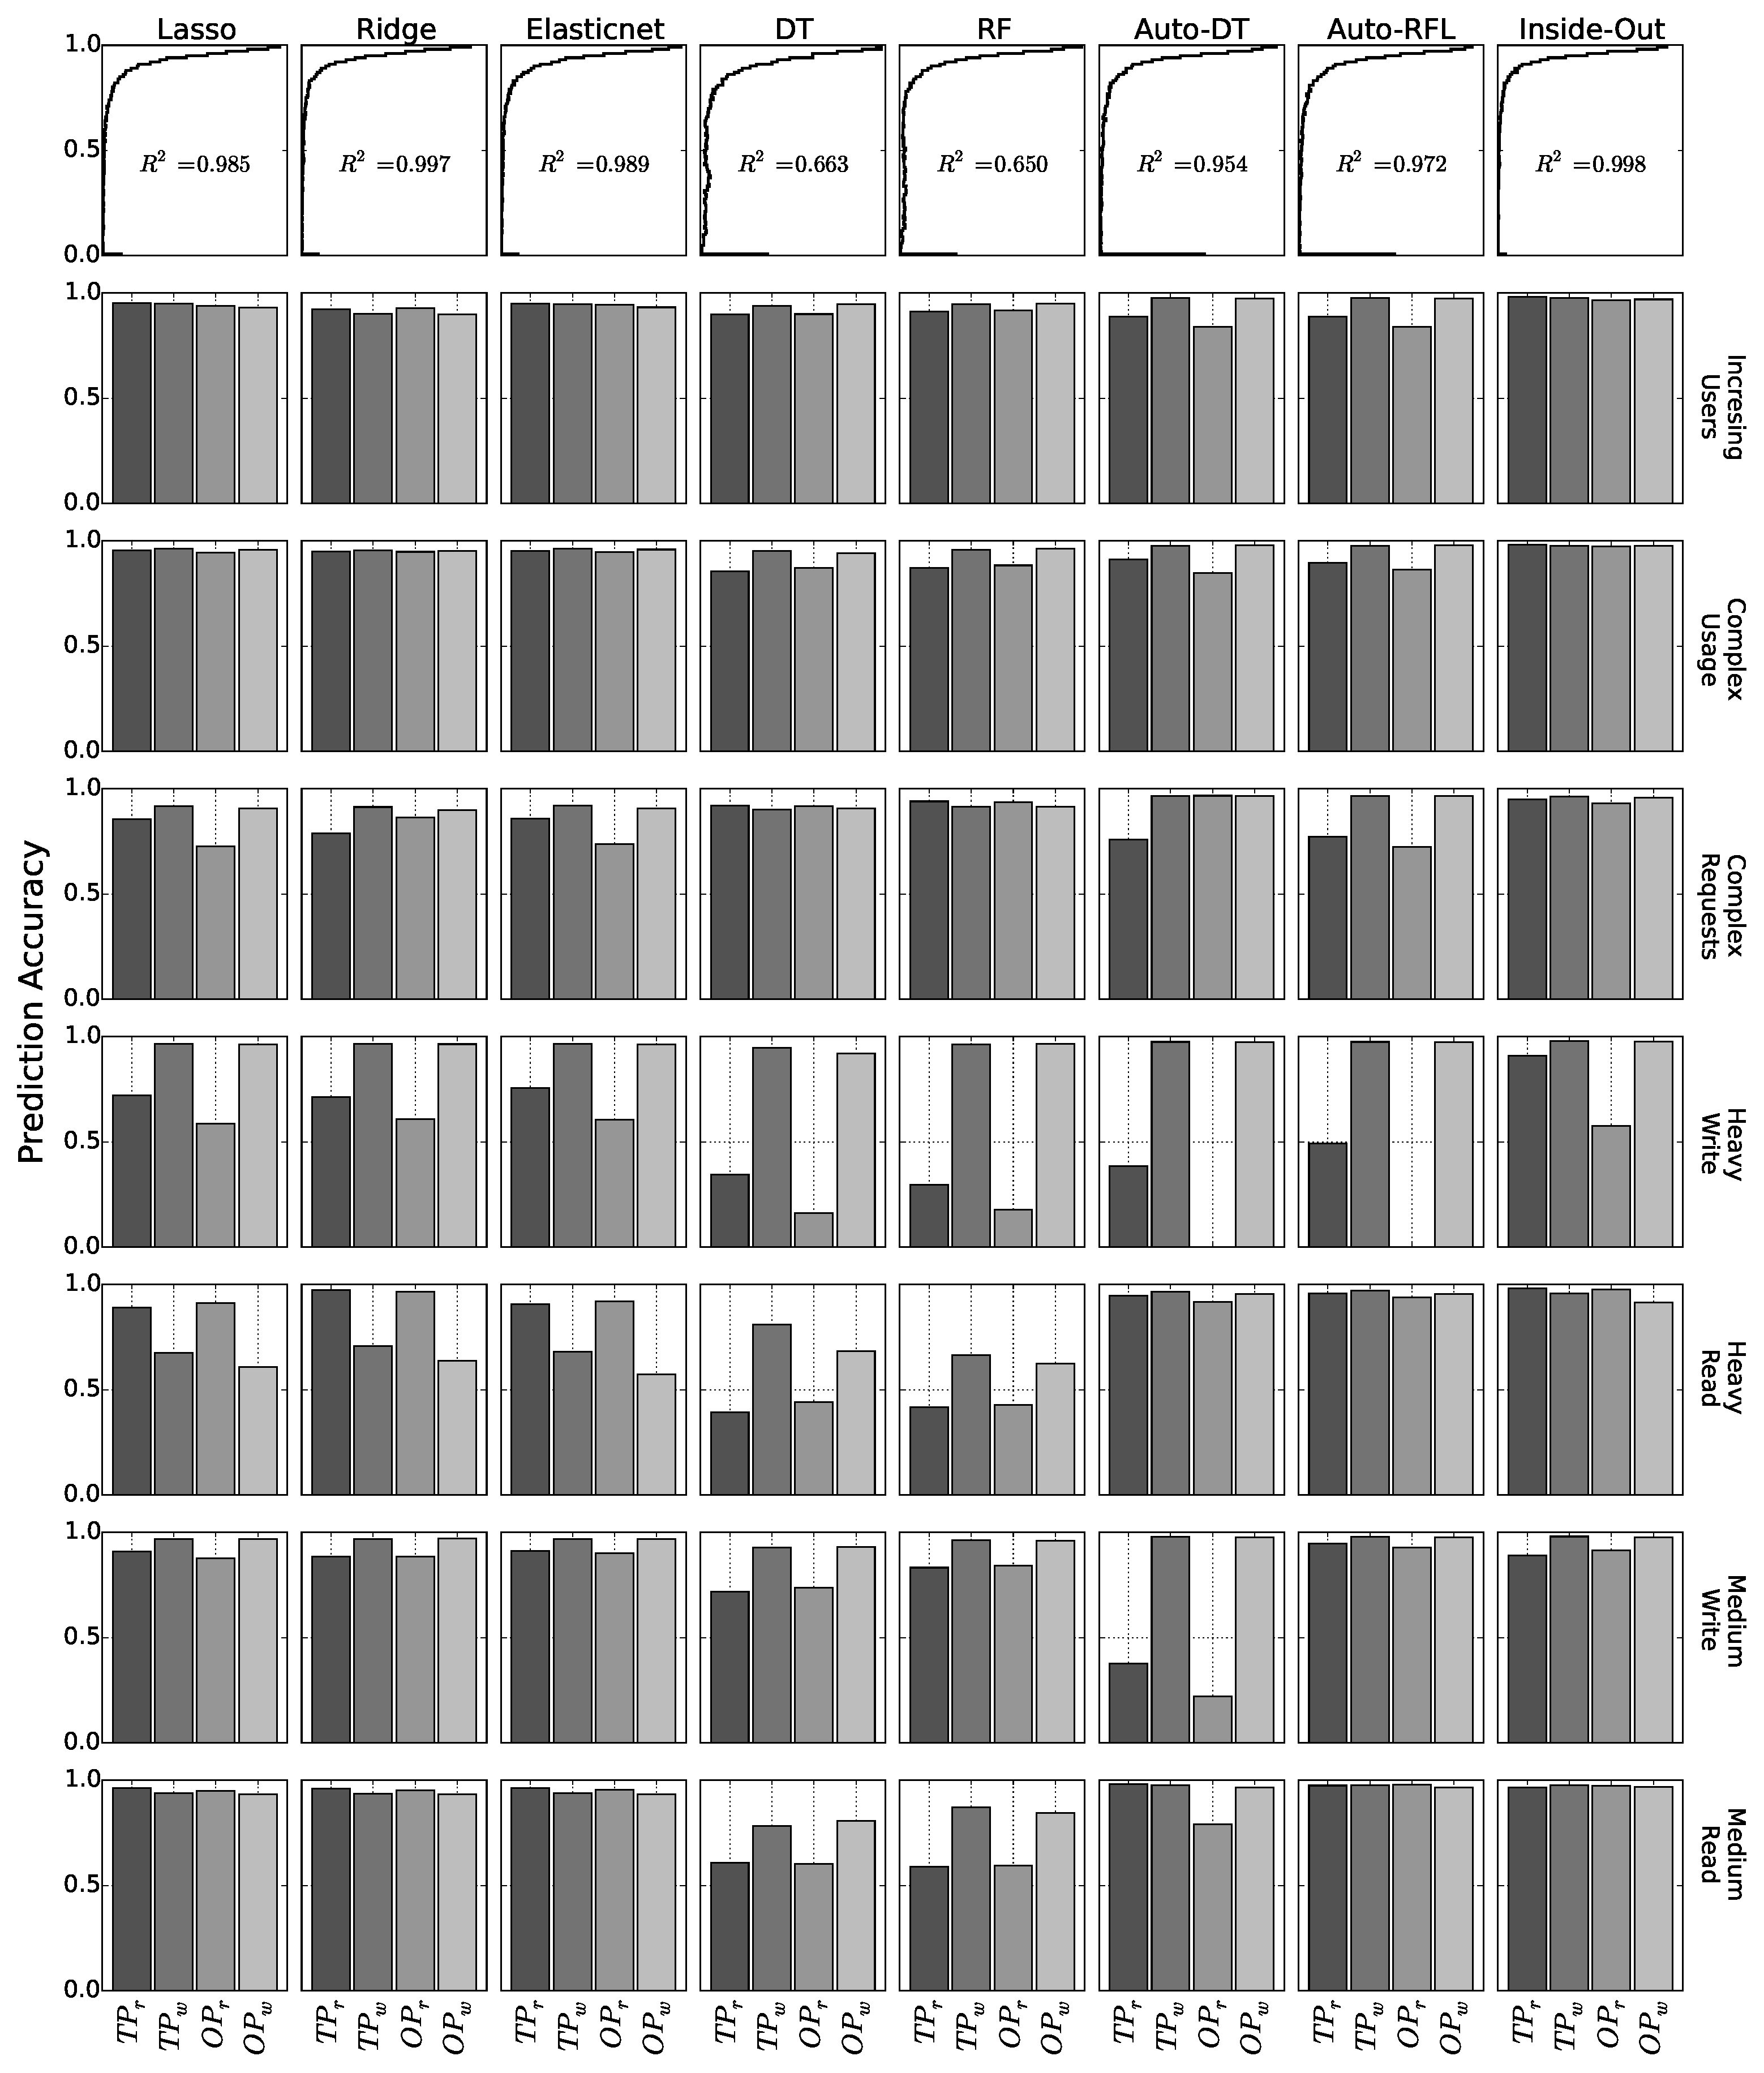
\includegraphics[width=0.9\textwidth]{Chapter-InsideOut/figures/unseen_workload_all_new.eps}
    \caption{Analysis of performance models with diverse workloads. Each bar is the average prediction accuracy. The top row is the probability density function of prediction accuracy for each performance model.}
    \label{fig:changing_workload}
\end{figure}

%\hfill\break

An SDS application needs to handle various request volumes, object/file sizes and different ratios of read/write workloads.
%In practice, it is difficult to obtain a training dataset that includes all access patterns.
First we examine whether Inside-Out can achieve accurate and consistent predictions when workload changes.


\paragraph*{Changing user behavior}
%\textbf{Changing user behavior.}

We increase the number of concurrent clients to stress the Ceph cluster.
%We push the Ceph cluster to a certain limit by increasing the parallelism of clients.
The \emph{\MakeLowercase{\scenarioMU}} scenario changes the number of COSBench clients and the \emph{\MakeLowercase{\scenarioCUB}} scenario increases the worker threads of each client.
As shown in \myfigure{\ref{fig:changing_workload}}, all prediction models perform well. The linear regression technique performs slightly better than the tree-based learning.
The linearly increasing load is well captured by linear models because of proportional change in low-level metrics.
When we switch to the \emph{\MakeLowercase{\scenarioCRB}} scenario, the variable request size slightly changes the behavior of Ceph, affecting prefetching and caching. 
We observe that the linear regression methods (Lasso, Ridge and Elastic Net) show drops in accuracy, e.g. 20\% in the $OP_r$ case; however, Inside-Out 
maintains good accuracy. 
The tree-based learning shows comparable predictions (5-10\% lower) with Inside-Out in these settings.



%\textbf{Complex request behavior.}
%Next, we change the workload from a constant IO request size to variable size.
%In this case, Inside-Out slightly improves the prediction accuracy over Lasso, %and outperforms the three linear models.
%Auto-DT and Auto-RFL show inconsistent prediction result with about 15\% %degradation of accuracy, comparing with the best case.
%One possible expalantion is that some important features filtered by DT and RF 
%are removed.
%Lasso and Elastic Net encounters accuracy drop in the read IOPS prediction


\paragraph*{Varying I/O pattern}

%The workload is a strong performance factor to a storage system \cite{Noorshams2013}.
%The read performance, for example, is affected by the amount of concurrent read or write operations.
Next, we consider workloads with different ratios of read to write operations.
\myfigure{\ref{fig:changing_workload}} shows that varying workload poses a big challenge to performance models. 
The linear regression methods (Lasso, Ridge and Elastic Net) present better prediction accuracy than tree-based models (DT, RL).
In addition, we observe that several models make poor predictions of $TP_r$ and $TP_r$.
The reason is that read behavior is largely affected by \textit{cache}, and large read variance contributes to low prediction accuracy.
Inside-Out performs consistently well, whereas the three linear regression techniques show accuracy drops.
One exception is the $OP_r$ prediction in the \textit{write-intensive} scenario even though $TP_r$ prediction is accurate.
As we will show later in Section~\ref{sec:online_learning}, \emph{over- and under-predictions} cause such behavior. 
The self-learning property of Inside-Out improves its prediction accuracy as it keeps learning the new storage behavior.


\begin{figure}
    \centering
    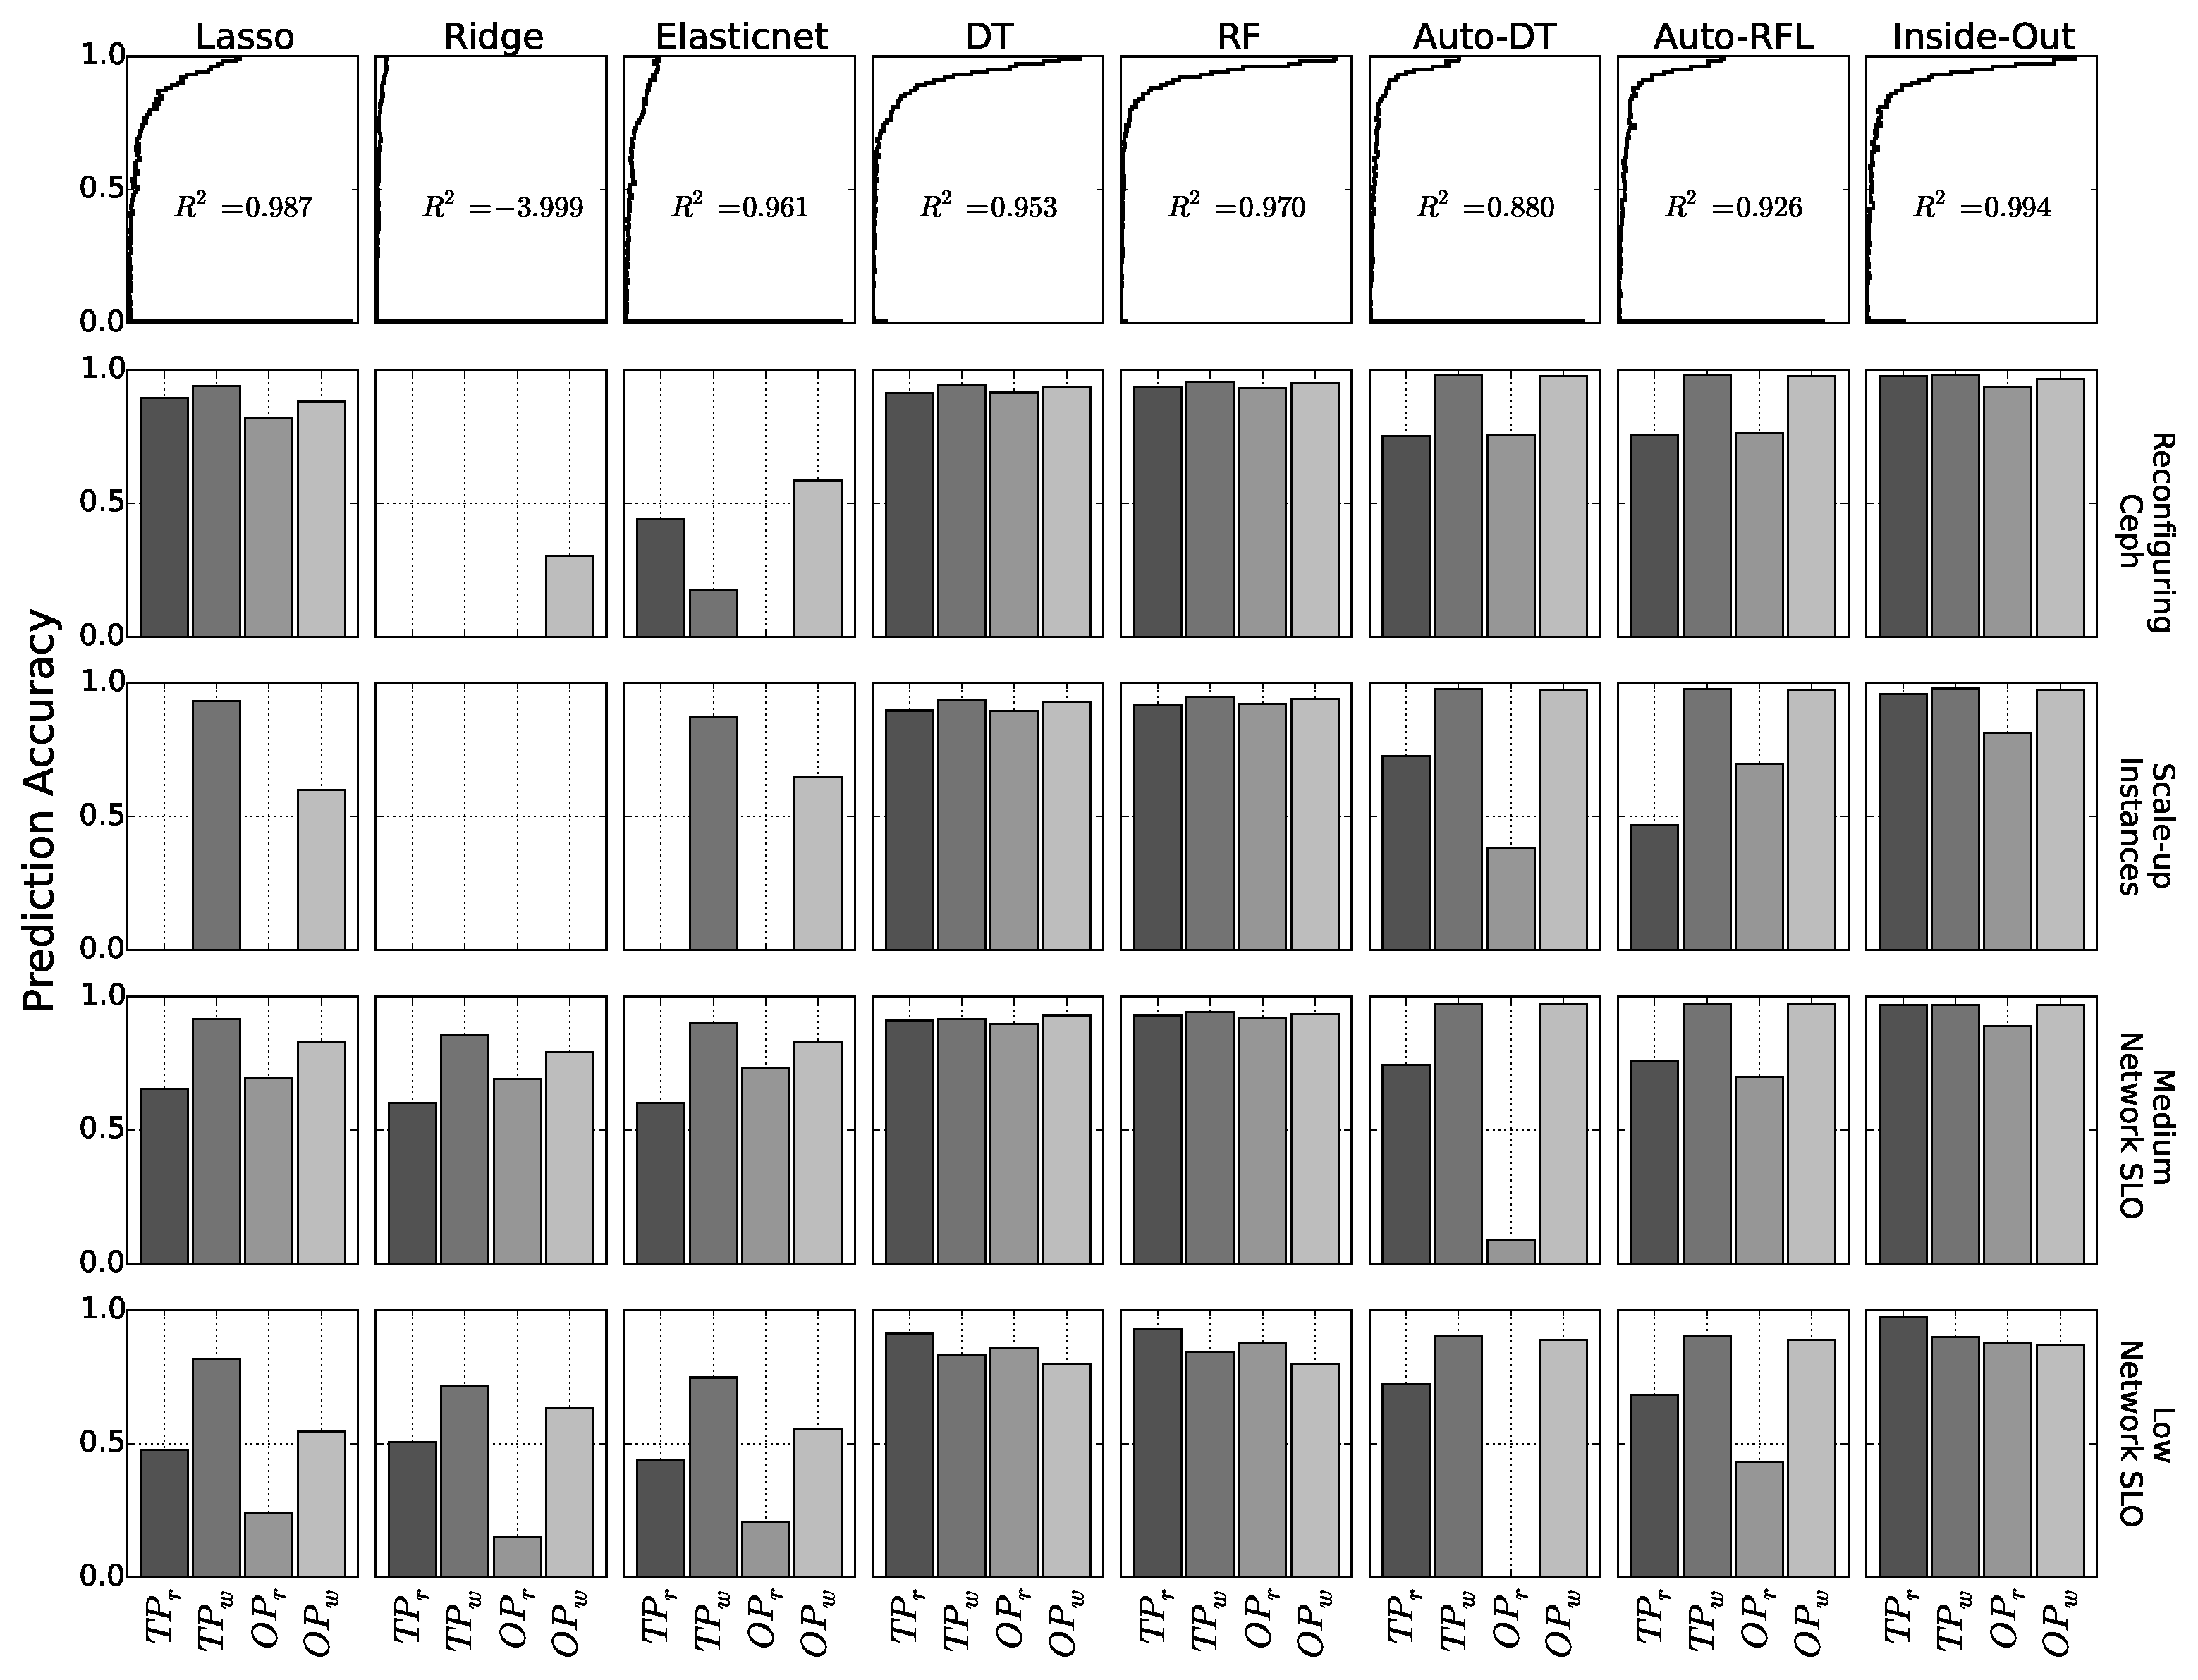
\includegraphics[width=0.9\textwidth]{Chapter-InsideOut/figures/unseen_configuration_all_new.eps}
    \caption{Comparison of performance models when the storage service is reconfigured: Ceph, VMs and network SLOs}
    \label{fig:reconfiguring_storage}
\end{figure}


\paragraph*{Summary}
The linear regression models achieve high prediction accuracy, great goodness-of-fit ($>0.98$) and consistency in prediction 
for many instances (see the distribution of prediction accuracy in \myfigure{\ref{fig:changing_workload}}), but they 
are not consistent across all prediction scenarios.
Inside-Out achieves good prediction accuracy across all cases consistently because the two-level approach 
filters out many irrelevant features in the first step, thereby presenting a smaller relevant feature space to the second step. 
The tree-based learning methods (DT and RF) do not show consistent prediction across all scenarios.
Auto-DT and Auto-RFL, which use DT and RF as the filter algorithms, are not as consistent as Inside-Out.

\vspace{1ex}

%\subsubsection{Reconfiguring Storage}
\subsubsection{Can Inside-Out handle different system configurations?}
\label{sec:unseen_configuration}

We study whether low-level metrics can capture the storage behavior when it is reconfigured by tenants. The results are reported in \myfigure{\ref{fig:reconfiguring_storage}}.


\textbf{Reconfiguring Ceph.}
The first change is to add one extra Ceph monitor daemon. %\chin{which increases the capability to handle a large number of clients.}
Ridge and Elastic Net fail to generate consistent predictions, but Lasso is able to achieve around 80\% to 90\% prediction accuracy.
DT, RF and Inside-Out have very close prediction accuracies, but Auto-DRL and Auto-RFL perform slightly worse in predicting $TP_r$ and $OP_r$.

\textbf{Scale-up instances.}
Increasing CPU and memory allocation to Ceph VM instances improves Ceph's ability to handle more requests.
In this test, we change the instance type from m1.small (1 vCPU, 2GB memory) to m1.medium (2 vCPUs, 4GB memory).
The linear models are unable to predict $TP_r$ and $OP_r$, but Inside-Out's two-level learning performs well by avoiding the overfitting problem. 

\textbf{Network SLOs.}
Here we consider the case where the amount of network bandwidth allocated to Ceph VMs is limited. 
We use Linux network throttling tool \textit{tc} to limit network bandwidth at 500 Mbps and 250 Mbps for medium and low bandwidth SLOs, respectively.
We observe that linear models without the two-level method do not show comparable prediction accuracy across both throughput and IOPS predictions.
The tree-based learning models, on the other hand, achieve 80\% to 90\% accuracy, comparable to Inside-Out.


\textbf{Summary.}
Tree-based learning (DT, RF) models demonstrate promising prediction in terms of prediction accuracy and consistency.
Lasso, Ridge and Elastic Net show inconsistent behavior in the above four scenarios.
Inside-Out, on the other hand, provides consistent predictions and improves Lasso, from 23.9\% to 87.6\% in the extreme case.


\begin{figure}
    \centering
    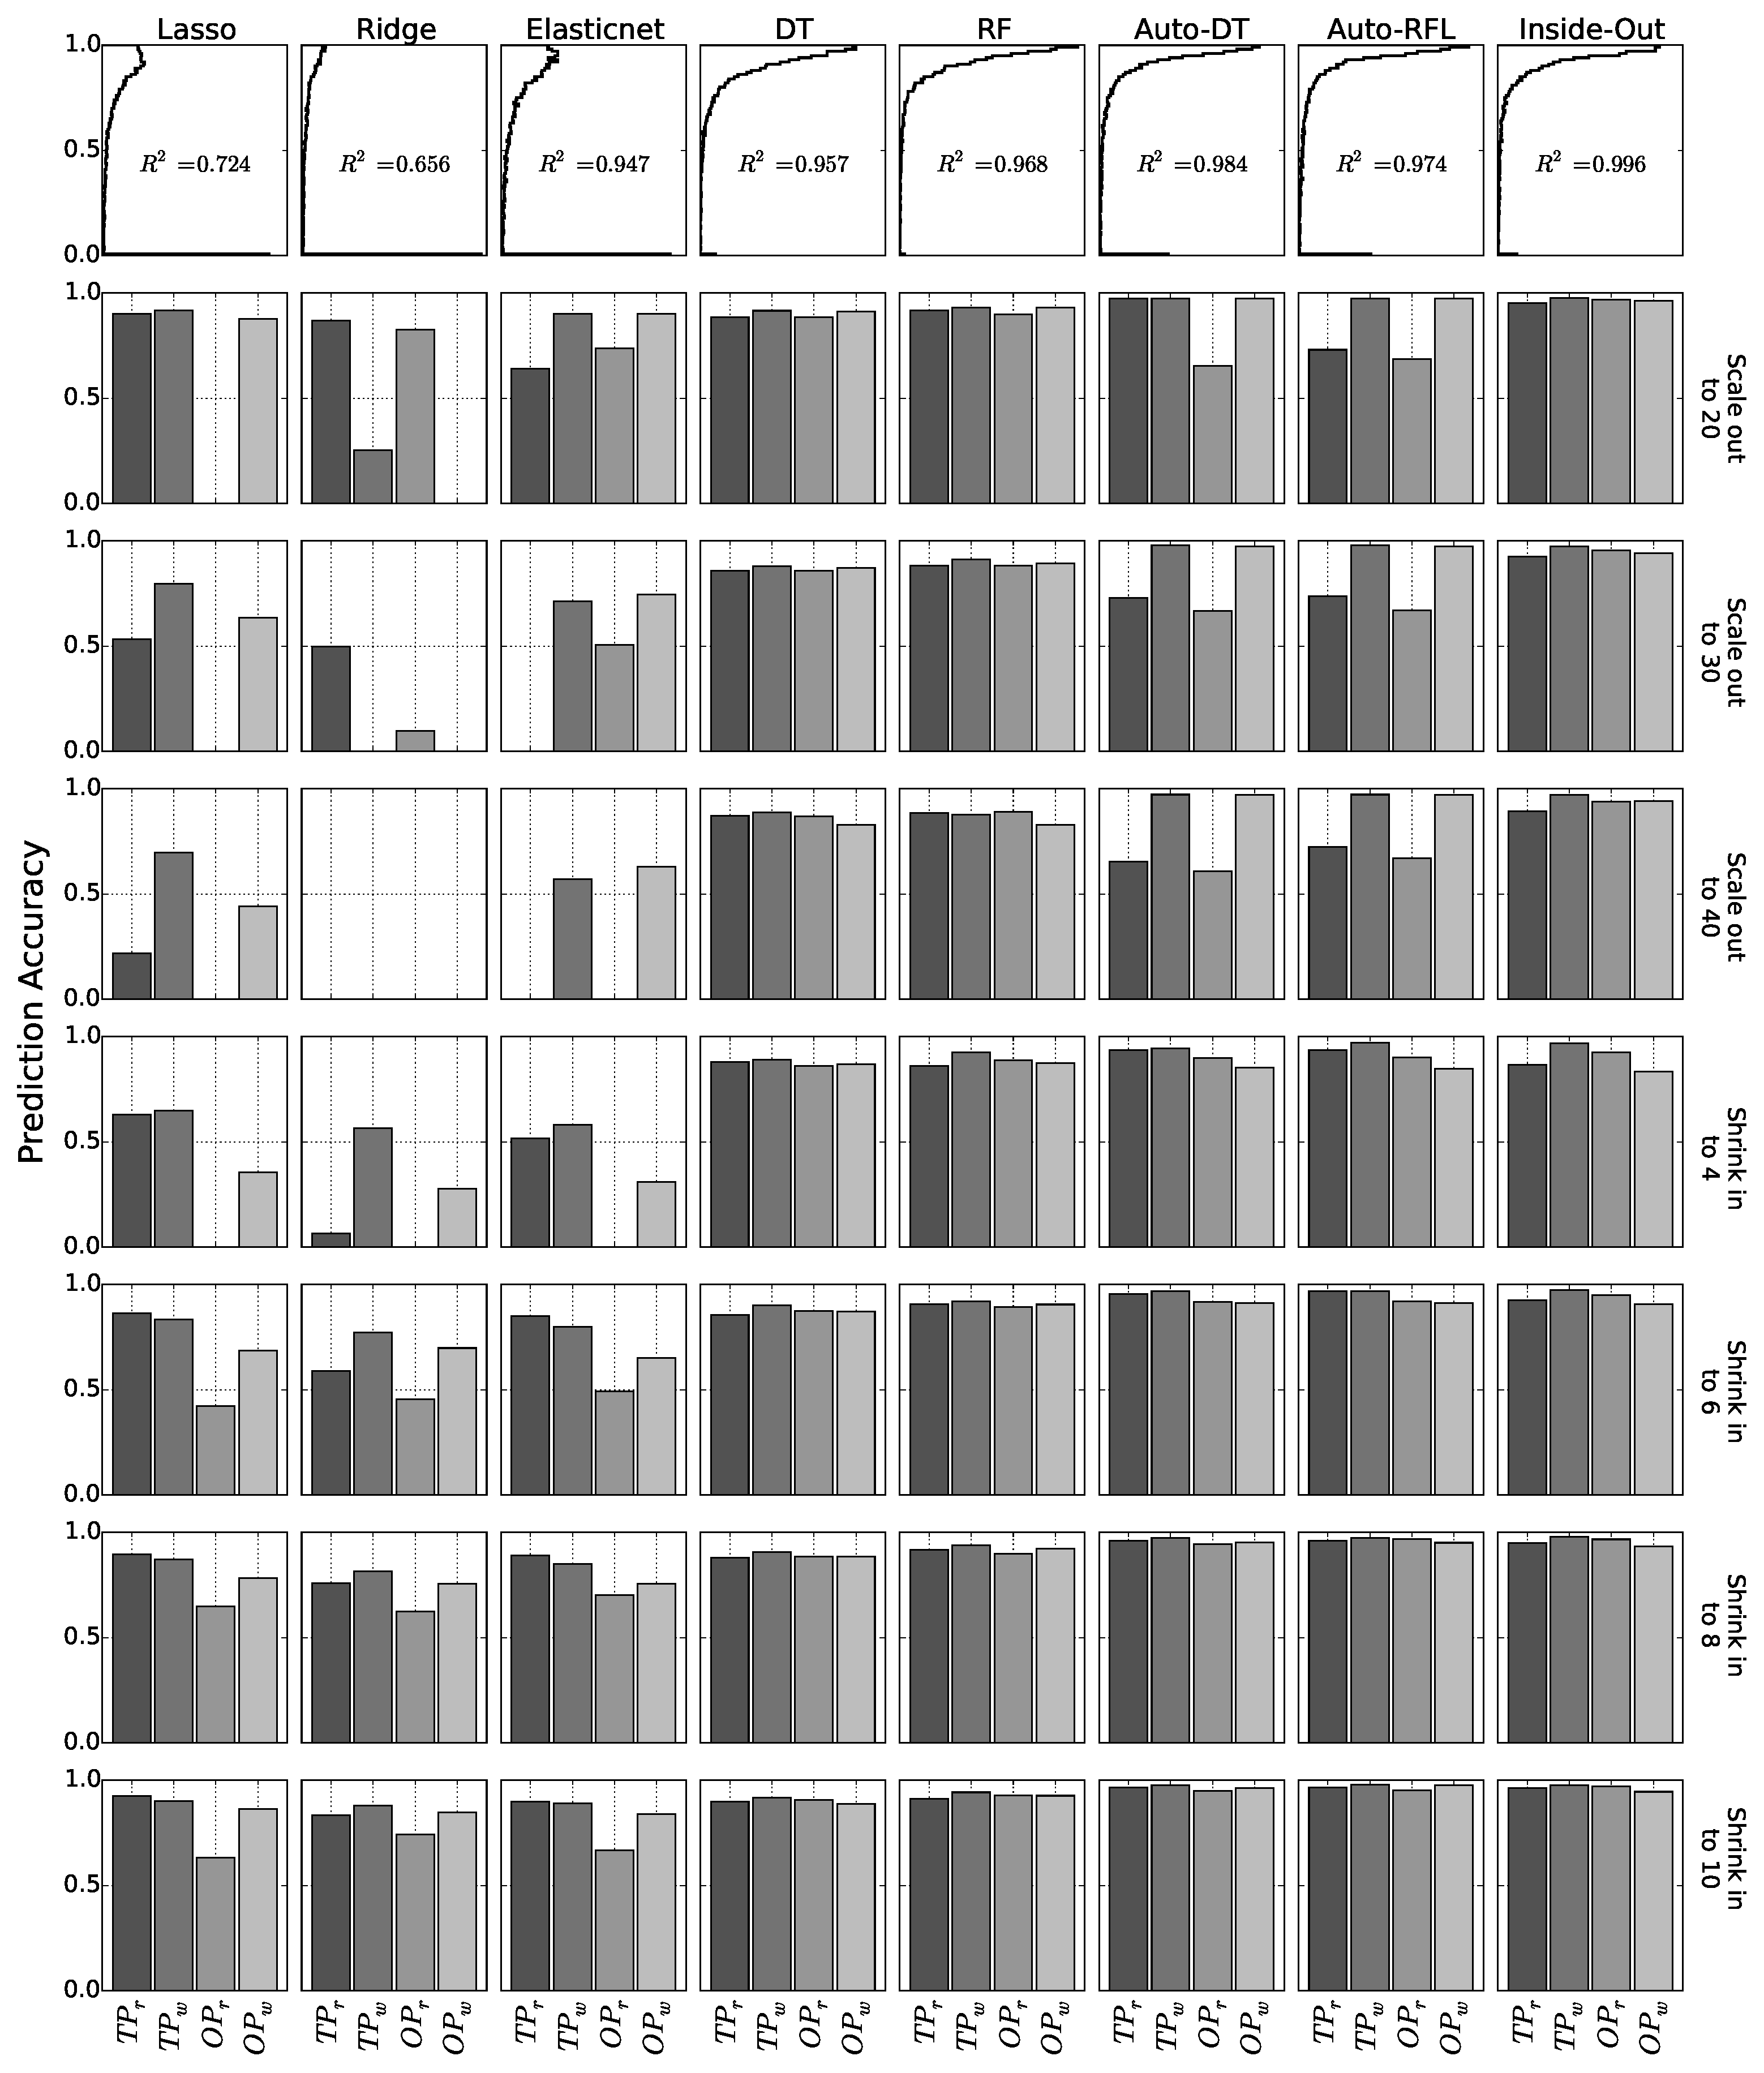
\includegraphics[width=0.9\textwidth]{Chapter-InsideOut/figures/unseen_scale_all_new.eps}
    \caption{Comparison of model performance in the on-demand scaling scenario. In the scale-out scenario, a performance model trained with 10 Ceph nodes is used to predict the performance of Ceph cluster with 20, 30 and 40 nodes.}
    \label{fig:elasticity}
\end{figure}


\subsection{Prediction Performance in a Multi-tenant Cloud}

This section examines the modeling performance of Inside-Out.
We first evaluate whether Inside-Out is able to extrapolate
performance of a larger Ceph cluster. 
Next, we evaluate how Inside-Out performs
when systems are subject to performance interference.

\subsubsection{Elastic Storage (On-demand Scaling)}
\label{sec:scaleout_prediction}

A storage service needs to grow or shrink its capacity on demand.
We evaluate Inside-Out's ability to capture the storage behavior at different system scales.
As shown in \myfigure{\ref{fig:elasticity}}, we use training data collected from 
4, 6, 8, and 10 nodes, and then predict the performance of 20, 30, and 40 nodes.
We also evaluate prediction accuracy in the \emph{shrink-in} scenario.
For both read and write throughput predictions, the linear models exhibit high variance.
In the $OP_r$ and $OP_w$ cases, the prediction results are not even comparable to the other methods.
Inside-Out, on the other hand, helps mitigate this issue, and achieves more than 90\% accuracy.
With increasing sizes of the storage, the prediction accuracy decreases because the prediction target 
becomes increasingly different from the training data.
Running a benchmark test against a very large system is time-consuming.
Here we demonstrate that Inside-Out can predict performance for systems that are 
four times larger than the system for which training data was collected.
%Due to resource limitations, we cannot show the upper bound of the largest system size that we can predict.
%However, we believe the upper bound can increase as the performance model keeps learning the system behavior.

\begin{figure}
    \centering
    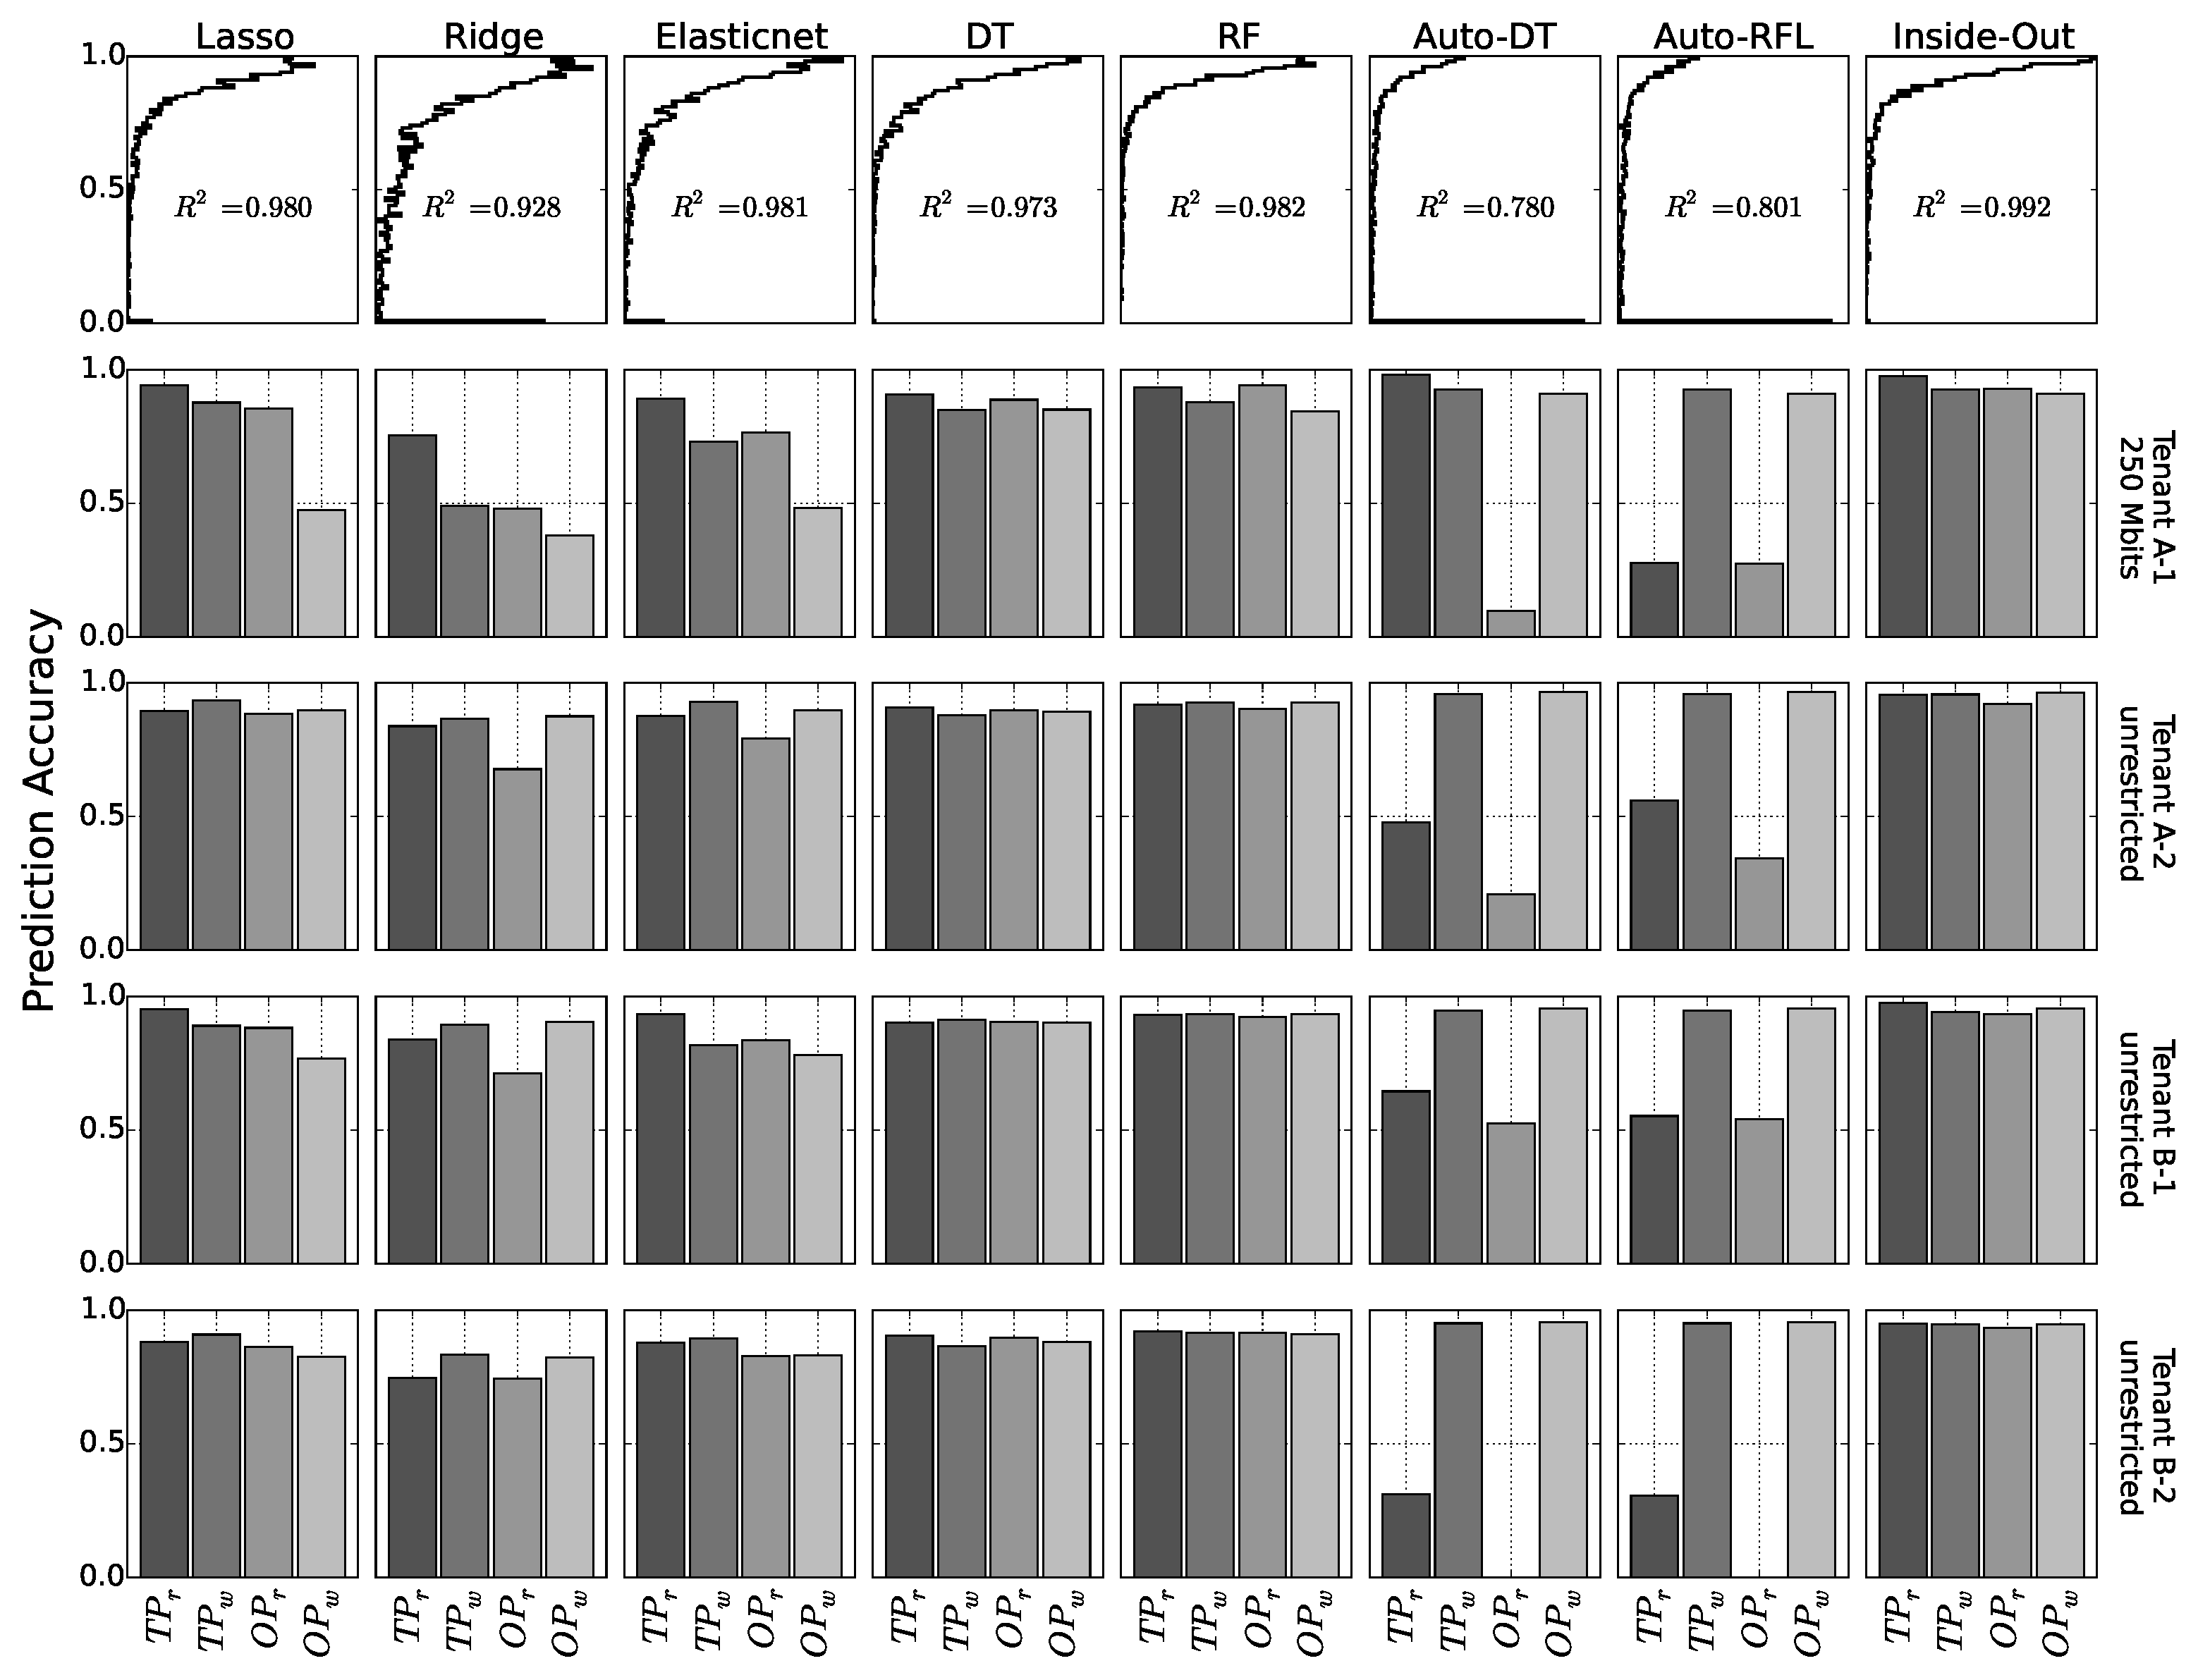
\includegraphics[width=0.9\textwidth]{Chapter-InsideOut/figures/multi_tenancy_all_new.eps}
    \caption{Prediction accuracy in a multi-tenancy scenario. Tenant A-1 is co-located with Tenant B-2. Tenant A-1 is throttled at 250Mbps. Tenant B-1 and B-2 are co-located without any traffic throttling.}
    \label{fig:multi_tenancy}
\end{figure}


\begin{figure*}
    \centering
    \includegraphics[width=0.9\textwidth]{Chapter-InsideOut/figures/real-world_tp_read.pdf}
    \caption{Application of Inside-Out to real time prediction of read throughput on a 10-node Ceph cluster.  Inside-Out starts from a simple prediction model trained by our collected benchmarking data.  Inside-Out keeps learning the storage behavior while improving prediction accuracy over time.}
    \label{fig:real_workload}
\end{figure*}


\subsubsection{Multi-Tenancy}
 
Next we evaluate Inside-Out's ability to adapt to performance interference among storage tenants.
We consider two cases for this evaluation. 
Each tenant runs a Ceph cluster with 10 OSDs separately, but tenants share the same 10 physical machines.
In the first case, we restrict the bandwidth of only the first tenant at 250Mbps.
%Two tenants compete for resources and \chin{\textbf{Tenant A-1}} has lower bandwidth SLO.
In the second case, we run two concurrent Ceph clusters but without network throttling.
\myfigure{\ref{fig:multi_tenancy}} shows that most prediction models are able to achieve more than 80\% accuracy.
The linear models like Ridge and Elasticnet yield lower prediction accuracies in some cases; however, Inside-Out performs well consistently.
Performance interference is challenging for a performance model designed for an isolated environment.
This evaluation demonstrates that the low-level performance metrics are good proxies for measuring
the end-to-end storage performance, even in a shared SDS environment.
%These metrics are able to reflect the behavior changes in the storage system.

%low-level performance feature selection approach is effective in capturing end-to-end performance, even under high storage interference.
%This property is important to SDS because it can help guarantee reliable end-to-end performance in a shared SDS environment.



\begin{comment}
\begin{figure*}
    \centering
    \includegraphics[width=0.9\textwidth]{figures/synthetic.eps}
    \caption{An online prediction scenario about six-hour long workload.  This synthetic workload is composed of 360 stages and each stage uniformly selects parameters such as workload types, request sizes and the number of clients.  The average stage duration is 60 seconds with standard deviation 20 seconds.}
\end{figure*}
\end{comment}

\begin{comment}
\begin{figure*}
    \centering
    \begin{subfigure}[b]{0.45\textwidth}
        \includegraphics[width=\textwidth]{figures/synthetic_read.eps}
        \caption{Read Throughput}
        \label{fig:synthetic_read}
    \end{subfigure}
    ~ %add desired spacing between images, e. g. ~, \quad, \qquad, \hfill etc.
      %(or a blank line to force the subfigure onto a new line)
    \begin{subfigure}[b]{0.45\textwidth}
        \includegraphics[width=\textwidth]{figures/synthetic_write.eps}
        \caption{Write Throughput}
        \label{fig:synthetic_write}
    \end{subfigure}
    \caption{An online prediction scenario about six-hour long workload.  This synthetic workload is composed of 360 stages and each stage uniformly selects parameters such as workload types, request sizes and the number of clients.  The average stage duration is 60 seconds with standard deviation 20 seconds.}
    \label{fig:synthetic_workload}
\end{figure*}
\end{comment}

%\subsection{Synthetic Workload}
\subsection{Online Self-Learning}
\label{sec:online_learning}

%Our goal is to apply Inside-Out to an online system so that SDS providers can guarantee the performance of a storage service hosted on their SDS platform.
%To evaluate this potential, 
Next, we create several synthetic workloads with mixed read/write ratios.
This synthetic workload spans 12 hours with 720 stages.
Each stage is 60-second long on average, with a standard deviation of 20 seconds.
We run four COSBench virtual machines for benchmarking and up to eight threads per COSBench client, with 10 Ceph OSDs and one monitor daemon.
We use Inside-Out to build an initial performance model with the training dataset described in Section~\ref{sec:dataset}.
\myfigure{\ref{fig:real_workload}} shows the prediction result for read throughput.
We can observe that the generated model can capture the overall trend, but suffers from over and under predictions.
This is because our training dataset is generated from a relatively clean environment, \ie the OS memory is flushed before any benchmarking process.
However, in the online prediction setting, cache is continuously consumed by non-stop client requests, which 
causes the real time storage behavior to be different from the training dataset.
With continuous monitoring of the performance of the storage service, 
we use Inside-Out to generate a new performance model at the sixth hour.
\myfigure{\ref{fig:real_workload}} shows that Inside-Out learns the new storage behavior and therefore, 
the over- and under-prediction issues are greatly mitigated.
%This evaluation demonstrates the potential of Inside-Out when applying it in an online system.
By continuously learning the storage behavior, SDS can accurately capture performance changes and therefore is able to provide reliable storage service.

%the problems due to over- and under-predictions are greatly mitigated.
%This evaluation demonstrates how Inside-Out can be used to continuously learn the storage behavior in an online system.


\begin{figure}
\centering
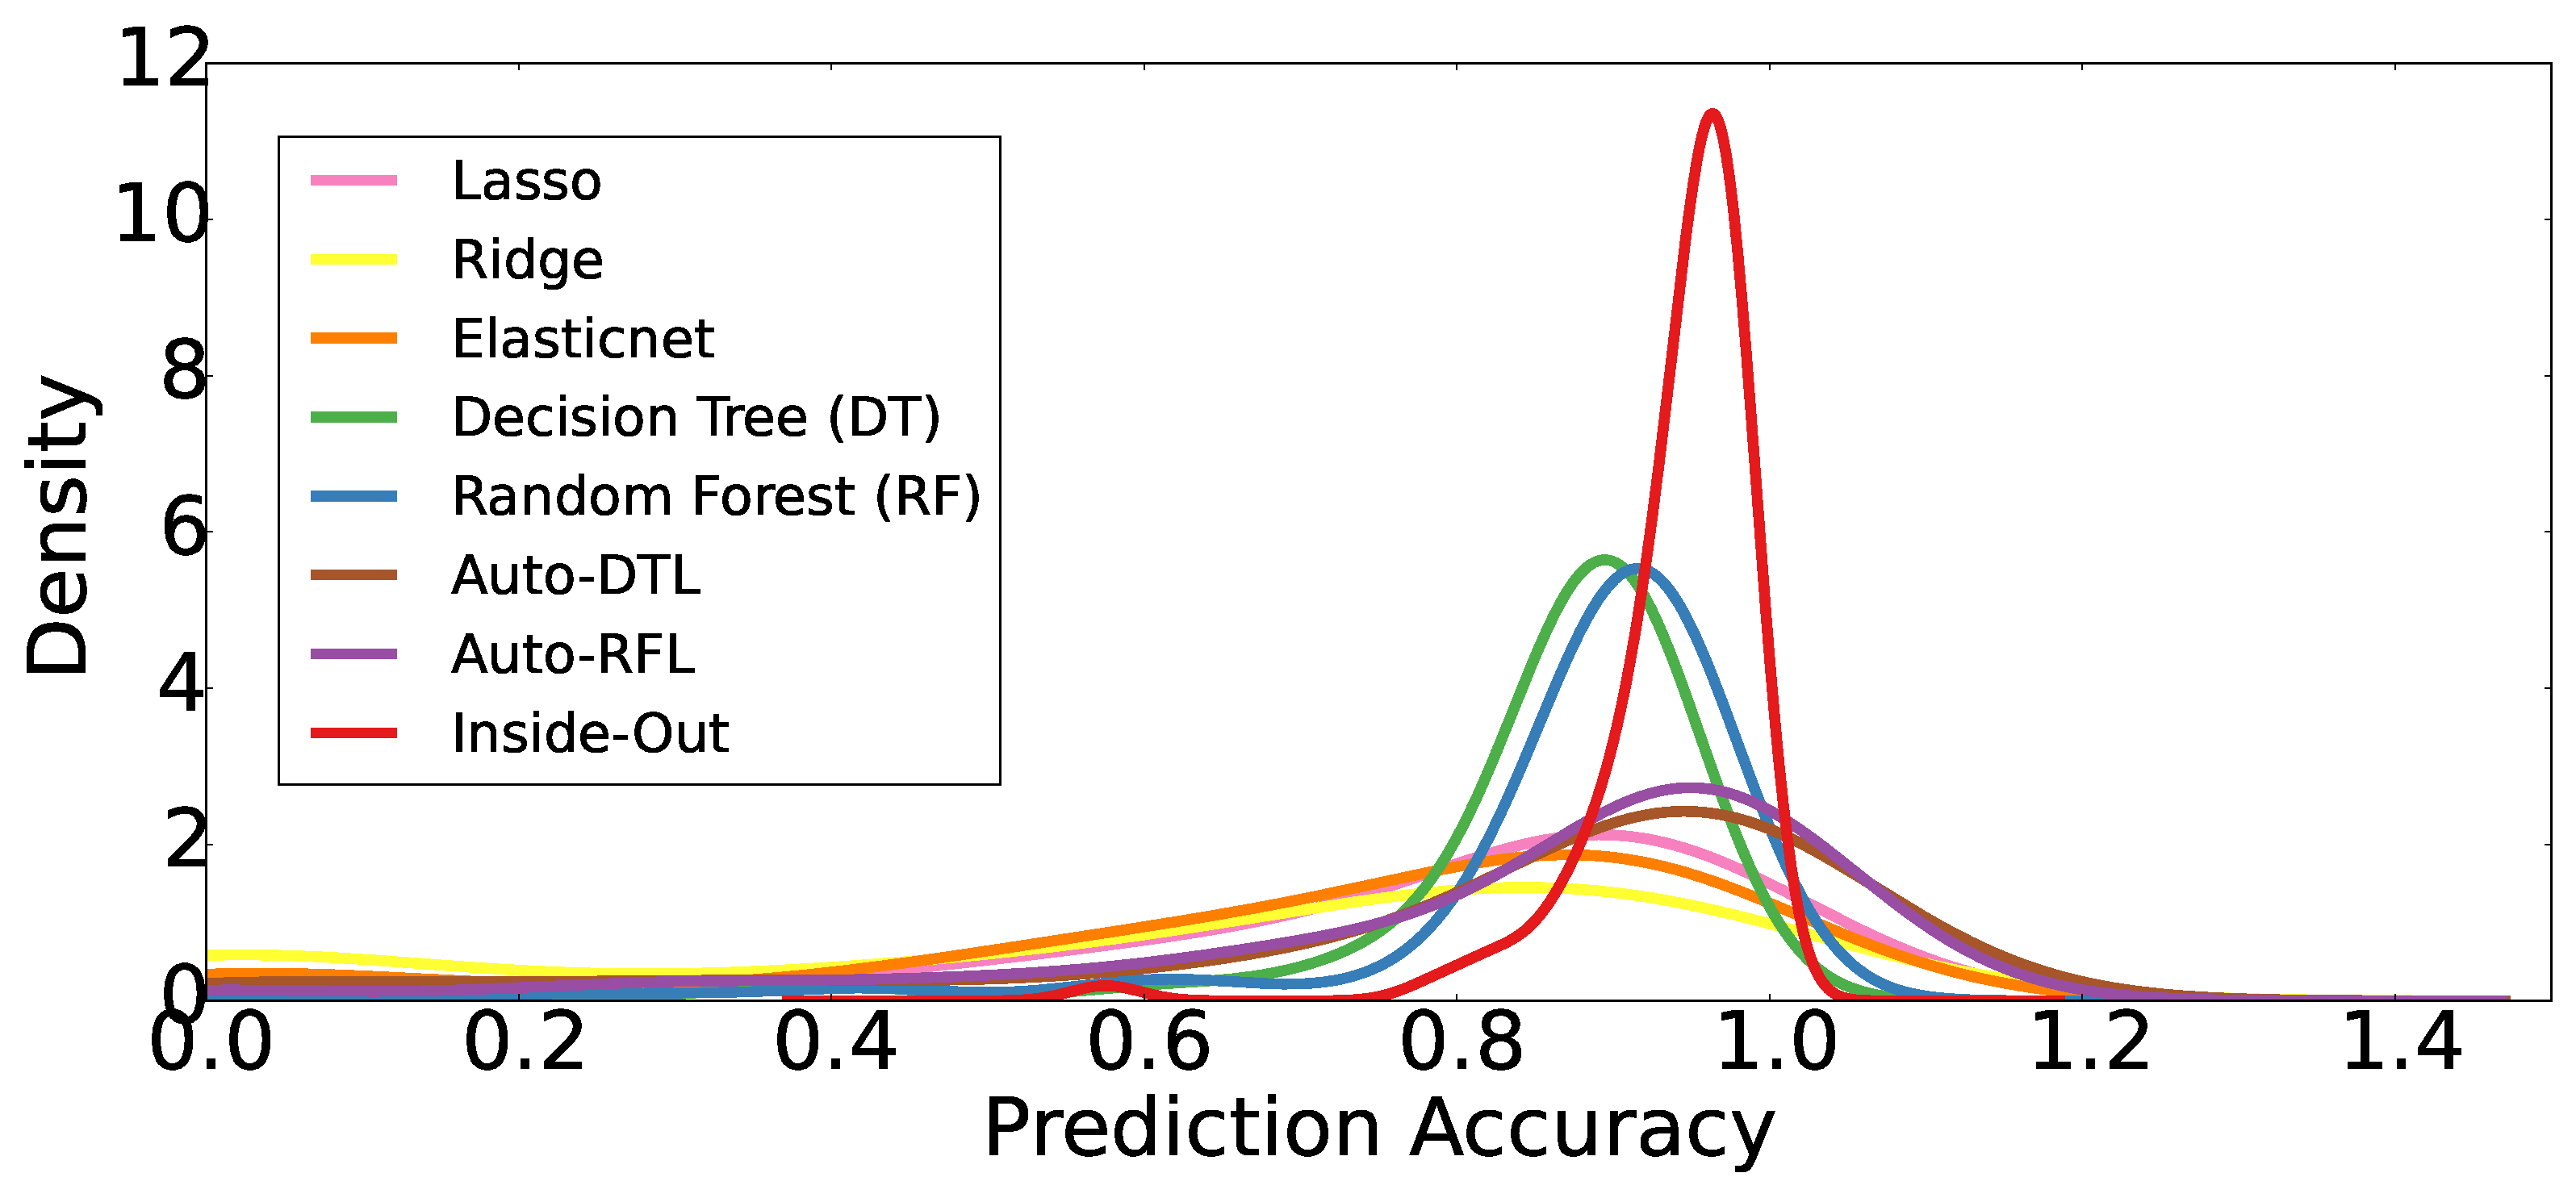
\includegraphics[width=0.9\textwidth, keepaspectratio]{Chapter-InsideOut/figures/aggregate_median.eps}
\caption{Kernel density function of prediction accuracy from \myfigure{\ref{fig:changing_workload}} to \myfigure{\ref{fig:multi_tenancy}}.  Each colored line represents the density function of a modeling approach.  Inside-Out is more consistent and accurate across almost every prediction case.}
\label{fig:aggregate}
\end{figure}


\vspace{1ex}
\subsection{Discussion}
We have shown that low-level performance metrics are useful to predict end-to-end throughput and IOPS.
%We applied Inside-Out to latency prediction and observe large variance and inconsistency.
%\chin{One} possible explanation is insufficient features and high variance in latency.
%The \chin{collected} low-level metrics are related to utilization, and these metrics might not provide enough information to fit a good model for predicting latency.
%Common approaches usually require request-level information \cite{Wang2004}.
%We need to further investigate latency prediction with other alternative generic low-level performance metrics.
Our evaluation has shown that low-level performance metrics are good indicators of end-to-end throughput and IOPS. 
Most existing performance models exhibit an inconsistent prediction behavior in the presence of diverse storage scenarios, 
such as changing workload, storage reconfigurations,
growing/shrinking storage, and multi-tenancy environments.
Our proposed two-level learning method can greatly improve prediction accuracy and yield consistent behavior.
Machine learning provides powerful tools, but they need to be used intelligently to achieve the best prediction accuracy. 
\myfigure{\ref{fig:aggregate}} shows the kernel density function of prediction accuracy across all prediction scenarios.
Inside-Out is a clear winner in terms of accuracy and consistency. 
More importantly, Inside-Out is able to learn new storage behavior, thereby enabling the performance model to adapt to the complex SDS environment.





% %\section{Related Work}
\label{sec:related_work}

\begin{itemize}
\item
  Characterizing application
\item
  Analyzing the energy-time trade-off in high-performance computing
  applications
\item
  Dynamically Controlling Node-Level Parallelism in Hadoop
\item
  Data-Driven Performance Modeling
\item
  Model Building

  \begin{itemize}
  \item
    Inside-out
  \end{itemize}
\item
  Configuration Recommendation
\item
  Parameter Tuning

  \begin{itemize}
  \item
    Selfish
  \item
    Dynamically Controlling Node-Level Parallelism in Hadoop
  \end{itemize}
\item
  Storage configurations
\item
  Cloud configurations

  \begin{itemize}
  \item
    Earnest
  \item
    CherryPick
  \end{itemize}
\item
  Search Algorithms
\item
  Random Search
\item
  Coordinate Descent
\item
  Genetic Algorithm
\item
  Bayesian Optimization
\end{itemize}
% \section{Conclusion}
\label{sec:conclusion}

The decoupled Hadoop model is flexible and much more preferable in many scenarios.
However, existing Hadoop schedulers do not consider this model and hence the scheduling method fails to optimize the system throughput.
Our flow scheduling method uses the penalty cost for task assignments in order to increase the processing flow rate on computing facilities.
We encode this problem as the min-cost flow problem and then we can obtain the optimal assignment.
We have implemented a pluggable Flow Scheduler for Hadoop YARN and it supports the latest version of Hadoop.
Our experiment results have shown that our flow scheduling can greatly improve the system throughput by about 30\% so as to eliminate stragglers.
These results support that the proposed flow scheduling can maintain the flow rate of processing.

Flow scheduling seems efficient for the decoupled model, but there still remains large space to improve.
For our current implementation, Flow Scheduler requires job profile and machine profile, which is not practical.
We believe we can estimate the flow demand of tasks and the flow capability of facilities at runtime.
A naive approach is to sample the flow demand of a task and then use this information to decide the cost of the remaining tasks of the same job.
Another approach is to monitor the flow rate of tasks so that we can adjust the penalty cost dynamically.
We can also decide the flow capability of facilities in a similar way.
Overall, we are positive about flow scheduling but more extensive evaluations have to be conducted before we can conclude.
